\documentclass[notes,10pt, aspectratio=169]{beamer}


\usepackage{pgfpages}
% These slides also contain speaker notes. You can print just the slides,
% just the notes, or both, depending on the setting below. Comment out the want
% you want.
\setbeameroption{hide notes} % Only slide
%\setbeameroption{show only notes} % Only notes
% \setbeameroption{show notes on second screen=right} % Both

\usepackage{import}
% \usepackage{helvet} %? to change the font to Helvetica
% \usepackage[default]{lato}
% \usepackage{verbatim}

\usepackage{array}
% \usepackage{natbib}
% \bibliographystyle{plain}
\usepackage{apalike}
\bibliographystyle{apalike}
% \usepackage[natbib, maxcitenames=3, mincitenames=11, style=apa]{biblatex}

% \usepackage{fontspec} %! error

% \usefonttheme{professionalfonts} % using non standard fonts for beamer
% \usefonttheme{serif} % default family is serif

% \setmainfont{Liberation Serif}

% \setsansfont{Liberation Serif}


\usepackage{tikz}
\newcommand*\circled[4]{\tikz[baseline=(char.base)]{
 \node[shape=circle, fill=#2, draw=#3, text=#4, inner sep=2pt] (char) {#1};}}



\setbeamertemplate{note page}{\pagecolor{yellow!5}\insertnote}
\usetikzlibrary{positioning}
\usetikzlibrary{snakes}
\usetikzlibrary{calc}
\usetikzlibrary{arrows}
\usetikzlibrary{decorations.markings}
\usetikzlibrary{shapes.misc}
\usetikzlibrary{matrix,shapes,arrows,fit,tikzmark}
\usepackage{amsmath}
\usepackage{mathpazo}
\usepackage{hyperref}
\usepackage{lipsum}
\usepackage{multimedia}
\usepackage{graphicx}
\usepackage{multirow}
\usepackage{graphicx}
\usepackage{dcolumn}
\usepackage{bbm}
\usepackage{cancel}
\newcolumntype{d}[0]{D{.}{.}{5}}
\usepackage{subcaption}
\usepackage{changepage}
\usepackage{appendixnumberbeamer}
\newcommand{\beginbackup}{
 \newcounter{framenumbervorappendix}
 \setcounter{framenumbervorappendix}{\value{framenumber}}
 \setbeamertemplate{footline}
 {
 \leavevmode%
 \hline
 box{%
 \begin{beamercolorbox}[wd=\paperwidth,ht=2.25ex,dp=1ex,right]{footlinecolor}%
% \insertframenumber \hspace*{2ex} 
 \end{beamercolorbox}}%
 \vskip0pt%
 }
 }
\newcommand{\backupend}{
 \addtocounter{framenumbervorappendix}{-\value{framenumber}}
 \addtocounter{framenumber}{\value{framenumbervorappendix}} 
}


\usepackage{graphicx}
\usepackage[space]{grffile}
\usepackage{booktabs}

% These are my colors -- there are many like them, but these are mine.
\definecolor{blue}{RGB}{70,160,205}
\definecolor{red}{RGB}{213,94,0}
\definecolor{yellow}{RGB}{240,228,66}
\definecolor{green}{RGB}{0,158,115}

% % Enviroments
% \newtheorem{defin}{Definition.}
% \newtheorem{teo}{Theorem. }
% \newtheorem{lema}{Lemma. }
% \newtheorem{coro}{C
% \begin{frame}{Modeling Choice}orolary. }
% \newtheorem{prop}{Proposition. }
% \theoremstyle{definition}
% \newtheorem{examp}{Example. }
% % \numberwithin{problem}{subsection} 

\hypersetup{
 colorlinks=false,
 linkbordercolor = {white},
 linkcolor = {blue} 
}

\newcommand\Fontvi{\fontsize{8.5}{7.2}\selectfont}

\newcommand\Fontx{\fontsize{10}{7.2}\selectfont}
%% I use a beige off-white for my background
\definecolor{MyBackground}{RGB}{255,253,218}

%% Uncomment this if you want to change the background color to something else
%\setbeamercolor{background canvas}{bg=MyBackground}

%% Change the bg color to adjust your transition slide background color!
\newenvironment{transitionframe}{
 \setbeamercolor{background canvas}{bg=white}
 \begin{frame}}{
 \end{frame}
}

\setbeamercolor{frametitle}{fg=blue}
\setbeamercolor{title}{fg=black}
\setbeamertemplate{footline}[frame number]
\setbeamertemplate{navigation symbols}{} 
\setbeamertemplate{itemize items}{-}
% \setbeamertemplate{itemize items}[circle]   
% \setbeamertemplate{itemize subitem}[triangle]
% \setbeamertemplate{itemize subsubitem}[circle]
% \setbeamertemplate{enumerate items}[default]
% \setbeamertemplate{section in toc}[circle]
% \setbeamertemplate{subsection in toc}[triangle]
% \setbeamertemplate{subsubsection in toc}[square]


\setbeamercolor{itemize item}{fg=blue}
\setbeamercolor{itemize subitem}{fg=blue}
\setbeamercolor{itemize subsubitem}{fg=blue}
\setbeamercolor{enumerate item}{fg=blue}
\setbeamercolor{enumerate subitem}{fg=blue}
\setbeamercolor{enumerate subsubitem}{fg=blue}
\setbeamercolor{button}{bg=MyBackground,fg=blue,}
\setbeamercolor{theotem}{fg=blue} 

% If you like road maps, rather than having clutter at the top, have a roadmap show up at the end of each section 
% (and after your introduction)
% Uncomment this is if you want the roadmap!
%\AtBeginSection[]
%{
% \begin{frame}
% \frametitle{Roadmap of Talk}
% \tableofcontents[currentsection]
% \end{frame}
%}

%  buttons transparent:
% \setbeamertemplate{button}{\tikz
%  \node[
%  inner xsep=10pt,
%  draw=structure!80,
%  fill=structure!50,
%  rounded corners=4pt]  {\insertbuttontext};}

\setbeamercolor{section in toc}{fg=blue}
\setbeamercolor{subsection in toc}{fg=red}
\setbeamersize{text margin left=1em,text margin right=1em} 

\newenvironment{wideitemize}{\itemize\addtolength{\itemsep}{10pt}}{\enditemize}

\usepackage{environ}
\NewEnviron{videoframe}[1]{
 \begin{frame}
 \vspace{-8pt}
 \begin{columns}[onlytextwidth, T] % align columns
 \begin{column}{.58\textwidth}
 \begin{minipage}[t][\textheight][t]
 {\dimexpr\textwidth}
 \vspace{8pt}
 \hspace{4pt} {\Large \sc \textcolor{blue}{#1}}
 \vspace{8pt}
 
 \BODY
 \end{minipage}
 \end{column}%
 \hfill%
 \begin{colußmn}{.42\textwidth}
 \colorbox{green!20}{\begin{minipage}[t][1.2\textheight][t]
 {\dimexpr\textwidth}
 Face goes here
 \end{minipage}}
 \end{column}%
 \end{columns}
 \end{frame}
}
% * Changing Font



% Unraveling Deposit Dynamics: Local Bank Competition and Segmented Deposit Markets

\title[]{\textcolor{blue}{The Digital Banking Revolution: \\
Effects on Competition and Stability}} %, Rate Dispersion and Profits in 

\subtitle{\textcolor{blue}{Naz Koont (2024)}\footnote{
    Stanford University, Graduate School of Business
}}
\author{Presenter: Giselle Labrador-Badia}
% university
\institute{University of Wisconsin-Madison}
%\centering
\date{\today}


\begin{document}
%%% TIKZ STUFF
\tikzset{ 
 every picture/.style={remember picture,baseline},
 every node/.style={anchor=base,align=center,outer sep=1.5pt},
 every path/.style={thick},
 }
\newcommand\marktopleft[1]{%
 \tikz[overlay,remember picture] 
 \node (marker-#1-a) at (-.3em,.3em) {};%
}
\newcommand\markbottomright[2]{%
 \tikz[overlay,remember picture] 
 \node (marker-#1-b) at (0em,0em) {};%
}
\tikzstyle{every picture}+=[remember picture] 
\tikzstyle{mybox} =[draw=black, very thick, rectangle, inner sep=10pt, inner ysep=20pt]
\tikzstyle{fancytitle} =[draw=black,fill=red, text=white]
%%%% END TIKZ STUFF

% % Title Slide
\begin{frame}[noframenumbering]
 \maketitle
\end{frame}



\begin{frame}{Introduction}

\begin{wideitemize}
    % \item Deregulation story: short until Riegle Act
    \item The Bank industry went through a deregulation process in the 1980s and 1990s.
    \vspace{0.2cm}
    \begin{wideitemize}
    \item In 1981 a bank could only operate in their home state or county.
    \item Deregulation process started in the 1980s with voluntary reciprocal interstate agreements.
    \item 1994 Riegle-Neal Act: banks could operate across state lines.
    \end{wideitemize}
    \pause
    \item \textcolor{blue}{Goal:} 
    % \item Preview of Results 
    \begin{wideitemize}
        \item Document the evolution of spatial sorting and expansion in response to deregulation.

        \item Provide a theory that rationalizes the observed patterns (framework Oberfield et al. (2024)).
        \begin{wideitemize}
            \vspace{0.2cm}
            % \item framework Of Oberfield et al. (2024) to generate sorting patterns:
            \item[1.] \textcolor{blue}{"Span-of-control sorting":} more productive banks sort into denser more expensive locations. %, while less productive banks sort into less attractive cheaper markets.
            \item[2.] \textcolor{blue}{"Mismatch sorting":} banks match the location's characteristics to the funding needs.
        \end{wideitemize}

    \end{wideitemize}


    \end{wideitemize}
    % \item Banks compete for deposits

   \end{frame}

   \begin{frame}{Introduction}

    \begin{wideitemize}
      
    
        \item   \textcolor{blue}{Contribution:} 
               \vspace{0.2cm}
        \begin{wideitemize}
            \item Theory that incorporates space and decision to locate branches.\footnote{Aguirregabiria et al. (2016, 2020), Corbae and E'Erasmos (2021,2021,2022) focus on diversification.}\footnote{Other recent papers are Ji et al (2023) and d'Avernas et al (2023).}
    
            \item Understanding location choice of bank through two forms of sorting: span-of-control and mismatch sorting.
        
            \item Literature of expansion of multi-plant firms \footnote{Rossi-Hansberg et al (2021), Hsieh and Rossi-Hansberg (2022)); international context: Antras et al (2017), Tintelnot (2016), and others.}
        \end{wideitemize}
        % \item Banks compete for deposits
    \end{wideitemize}
       \end{frame}


    
        \begin{frame}{Data}
    
    \begin{wideitemize}
        \item Bank branches and deposits from the FDIC (SOD) from 1981 to 2006.
      \begin{itemize}
            \item county as the geographical unit of analysis
        \end{itemize} 
        \item Bank-level wholesale funding from Call Reports
        \begin{itemize}
            \item time deposits, FR funds, brokered deposits.
        \end{itemize}
        \item  Aggregate to holding companies.
    
        \item County-level data on population and income from the Census and BEA.
    \end{wideitemize}
    
            \end{frame}
    
    

   % frame with figure

\begin{frame}{Basic Pattern: Fewer banks with many more branches}

\begin{figure}
    \centering
    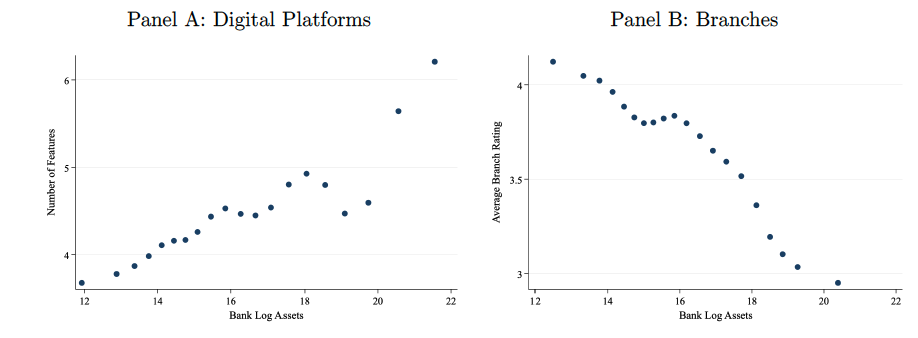
\includegraphics[width=0.99\textwidth]{imgs/fig3.png}
    % \caption*{Caption}
    \label{fig:my_label}
\end{figure}

\end{frame}

\begin{frame}{Basic Pattern: Top banks expanded by growing geographically}

    %We next highlight the nature of bank branch expansion across the bank size distribution. For a given size group $g$, in terms of total deposits, we first calculate the total number of branches in each size group. We then separate growth in the number of branches into an intensive and extensive margin, namely,
    For size group $g$, in terms of total deposits, branch growth is:
$$
\Delta \log \left(\text { branches }_{g t}\right)=\underbrace{\Delta \log (\text { branches per county })_{g t}}_{\text {intensive margin growth }}+\underbrace{\Delta \log (\text { counties })_{g t}}_{\text {extensive margin growth }} .
$$

%The variable counties $_{g t}$ is the total number of active counties across banks in size group $g$ in year $t$. The intensive margin component measures changes in the number of branches per active county for banks in
    \begin{figure}
        \centering
        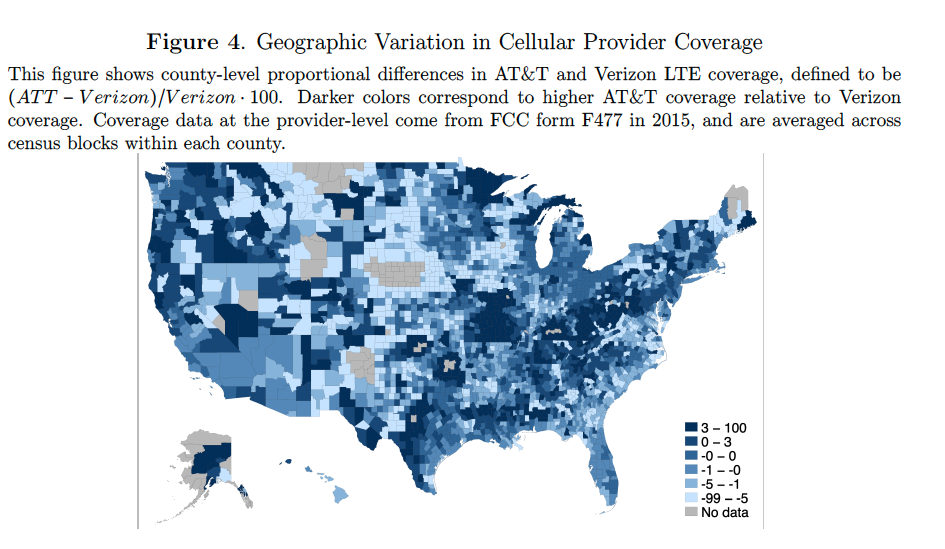
\includegraphics[width=0.92\textwidth]{imgs/fig4.png}
        %\caption*{Caption}
        \label{fig:my_label}
    \end{figure}
    
    \end{frame}

    \begin{frame}{Basic Pattern: Large banks use more wholesale funding}

        % Figure 6b documents the distribution of wholesale funding exposure, WFE, across banks in each size bin. We measure WFE as the ratio of a bank's wholesale funds to their retail deposits, that is, ${ }^{23}$
Wholesale funding exposure, WFE, across banks in each size bin:
        $$WFE_{bt} = \frac{FF_{bt} + TD_{bt} + BrokD_{bt}}{\text{Retail Deposits}_{bt}}$$
        
        \begin{figure}
            \centering
            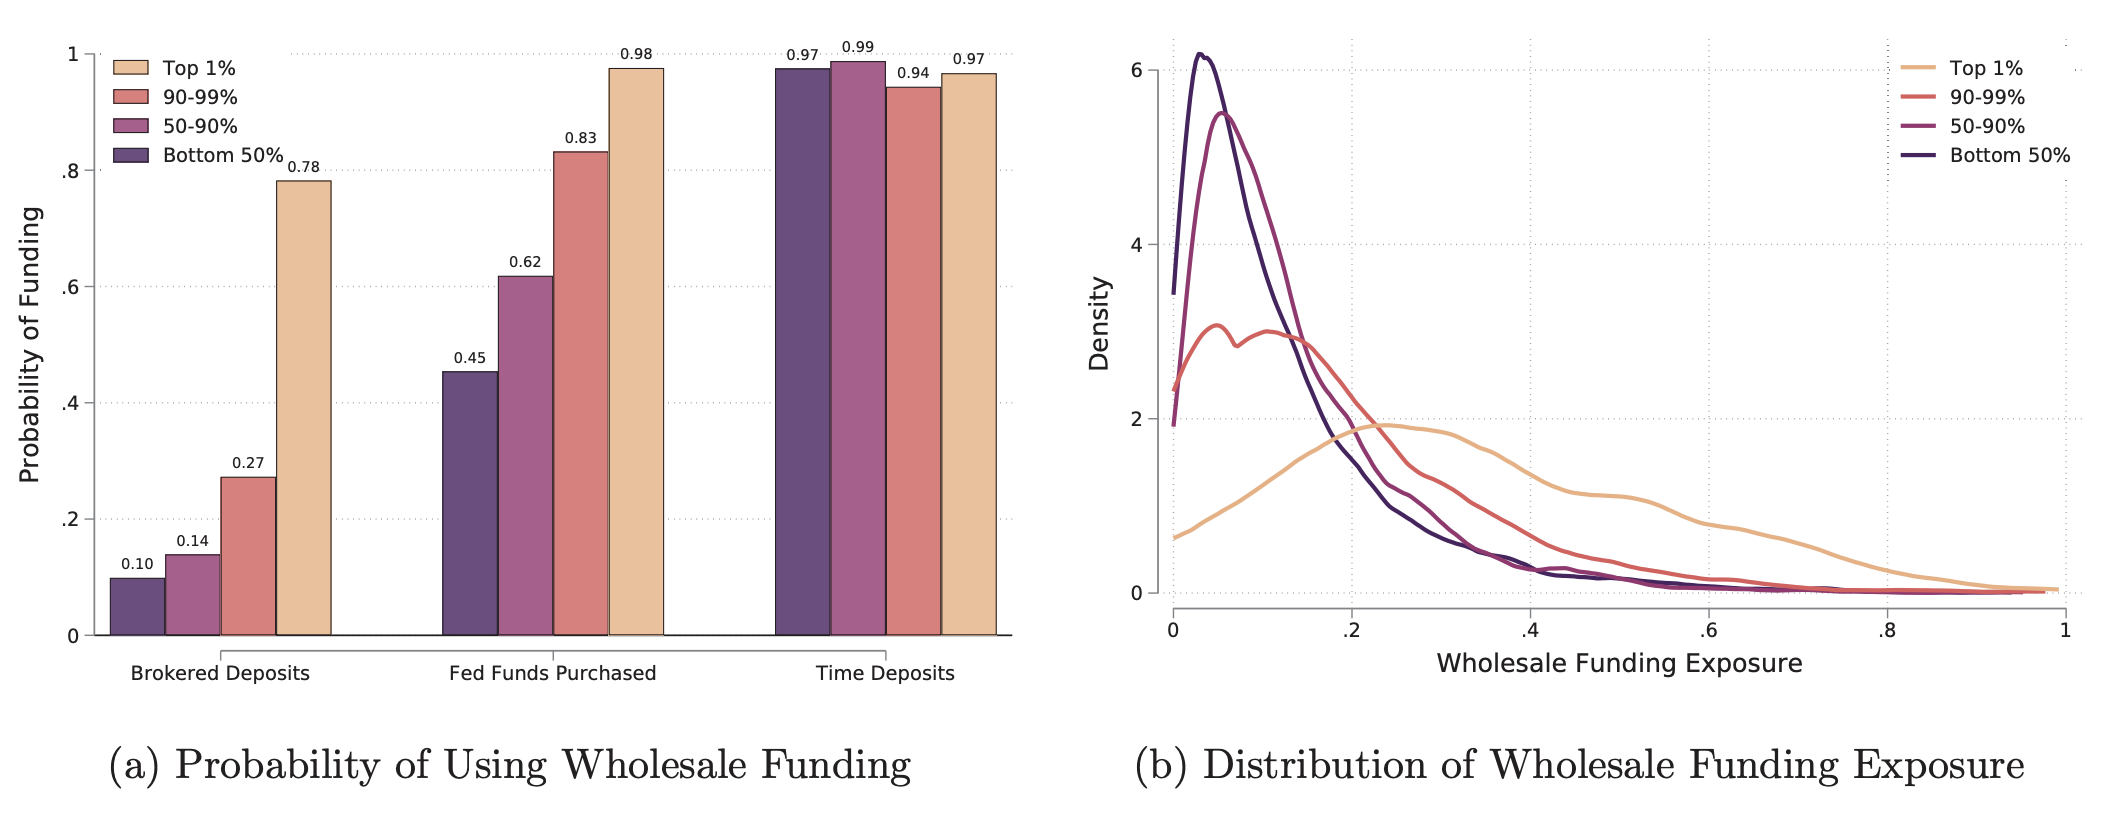
\includegraphics[width=0.9\textwidth]{imgs/fig6.png}
            \caption*{ The use of wholesale funds across the bank size distribution in 1984.}
            \label{fig:my_label}
        \end{figure}
        
        \end{frame}
% ********************************************************************************************************************


\begin{frame}[noframenumbering]

\huge \centering \textcolor{blue}{A Spatial Theory of Banking}

\end{frame}
    
\begin{frame}{Households}

    \begin{wideitemize}
        \item  Each location $\ell$ is composed of a set households $I_{\ell}$.
        % \item Heterogeneous households choose a bank and branch for loans and deposits 
        % \item Households have heterogeneous tastes for banks.   
        \item \textbf{Heterogeneous households} choose \text{bank} $j$ and \text{branch} $o^D_{j \ell} \in O_j$ for deposits, and 
        bank $k$ and branch $o^L_{k \ell}$ for loans,
        
        \item given distance to branch and rates $r_{j, o_{j \ell}^D}^D$ and $r_{k, o_{k \ell}^L}^L$,

        % \item Given all banks' location choices and interest rate choices, the residual demands are:
        % $$\begin{gathered}D_{j \ell}=T^D\left(\delta_{o_{j \ell}^D, \ell}\right) Q_{j \ell}^D A_{\ell}^D \mathcal{D}\left(r_{j, o_{j \ell}^D}^D\right), \\ L_{j \ell}=T^L\left(\delta_{o_{j \ell}^L, \ell}\right) Q_{j \ell}^L A_{\ell}^L \mathcal{L}\left(r_{j, o_{j \ell}^L}^L\right) .\end{gathered}$$

        \item  common taste for bank $j$ deposit $Q_{j \ell}^D$ and loan $Q_{j \ell}^L$  in $\ell$: 
\begin{equation}
Q_{j \ell}^D=\bar{Q}_j^D J_{j \ell}^D \phi_{j \ell}
\end{equation}
\begin{equation}
Q_{j \ell}^L=\bar{Q}_j^L J_{j \ell}^L \phi_{j \ell},
\end{equation}

        \begin{itemize}
            \item $\bar{Q}_j^D$ and $\bar{Q}_j^L$ are common for bank $j$ (from bank's investment decisions), 
            \item $J_{j \ell}^D$ and $J_{j \ell}^L$ are decreasing functions of distance to bank $j$ 's headquarters, 
            \item $\left\{\phi_{j \ell}\right\}_{\ell}$ are idiosyncratic appeal shifters drawn from a multivariate Frechet distribution.
        \end{itemize}

%where $\bar{Q}_j^D$ and $\bar{Q}_j^L$ are common for bank $j$ across all locations and will be determined by a bank's investment decisions; $J_{j \ell}^D \equiv J^D\left(\delta_{\ell}^{H Q}, \ell\right)$ and $J_{j \ell}^L \equiv J^L\left(\delta_{\ell_j^{H Q}, \ell}\right)$ where $J^D(\delta)$ and $J^L(\delta)$ are weakly decreasing functions of distance, to allow for the possibility that appeal is lower for locations further from bank $j$ 's headquarters at $\ell_j^{H Q} ;$ and $\left\{\phi_{j \ell}\right\}_{\ell}$ are idiosyncratic appeal shifters drawn from a multivariate Frechet distribution. ${ }^{26}$

    \end{wideitemize}

\end{frame}

\begin{frame}{ Households}

    \begin{wideitemize}

        \item Given all banks' location choices and interest rate choices, the \textbf{residual demands} are:
        \begin{equation}D_{j \ell}=T^D\left(\delta_{o_{j \ell}^D, \ell}\right) Q_{j \ell}^D A_{\ell}^D \mathcal{D}\left(r_{j, o_{j \ell}^D}^D\right)
        \end{equation}
        \begin{equation} L_{j \ell}=T^L\left(\delta_{o_{j \ell}^L, \ell}\right) Q_{j \ell}^L A_{\ell}^L \mathcal{L}\left(r_{j, o_{j \ell}^L}^L\right) \end{equation}

        \begin{wideitemize}
            \item $Q_{j \ell}^D$ and $Q_{j \ell}^L$ are common taste for bank $j$ deposit and loan services,
            \item $T^D(\delta)$ and $T^L(\delta)$ are decreasing functions of distance $\delta$,
            \item $A_{\ell}^D$ and $A_{\ell}^L$ are local demand shifters common to all banks (local population, local demand for deposits/loans, and local price levels/competition), 
        
            \item $\mathcal{D}\left(r_{j, o_{j \ell}^D}^D\right)$ and $\mathcal{L}\left(r_{j, o_{j \ell}^L}^L\right)$ is the impact of interest rates on demand.
            
            % summarizes the impact of interest rates on household-level demand for deposits and loans, incorporating both the impact of the interest rate on the probability of choosing to use a particular bank and on the amount of deposits and loans conditional on choosing that bank.

        \end{wideitemize}

    \end{wideitemize}


    \end{frame}

\begin{frame}{ Households}

    \begin{wideitemize}
        

        \item Given all banks' location choices and interest rate choices, the \textbf{residual demands} are:
        $$\begin{gathered}D_{j \ell}= \textcolor{blue}{T^D\left(\delta_{o_{j \ell}^D, \ell}\right)}  \textcolor{green}{Q_{j \ell}^D }\textcolor{red}{A_{\ell}^D} \mathcal{D}\left(r_{j, o_{j \ell}^D}^D\right) .\end{gathered}$$ %
        % , \\ L_{j \ell}=T^L\left(\delta_{o_{j \ell}^L, \ell}\right) Q_{j \ell}^L A_{\ell}^L \mathcal{L}\left(r_{j, o_{j \ell}^L}^L\right)



    \textcolor{blue}{Microfundation (Appendix)}:
    \vspace{0.3cm}
        \begin{wideitemize}
            \item From discrete choice model where households choose to bank and branch with idiosyncratic T1EV $\varepsilon_{ij}$. 
\begin{equation*}
D_{j \ell}  =\frac{e^{\eta\left[G^D\left(r_{j o_{j \ell}^D}^D\right)+ \textcolor{green}{\tilde{Q}_{j \ell}^D }\textcolor{blue}{-\tilde{T}^D\left(\delta_{\ell_{j \ell}^D}\right)}\right]}}{ \textcolor{red}{\sum_k e^{\eta\left[G^D\left(r_{k o_{k \ell}^D}^D\right)+\tilde{Q}_{k \ell}^D-\tilde{T}^D\left(\delta_{\ell_{k \ell}^D}\right)\right]}}}  \textcolor{red}{\int_{i \in I_{\ell}} \mathfrak{d}_i }\tilde{\mathcal{D}}\left(r_{j, o_{j \ell}^D}^D\right) \textcolor{red}{ d i }% \\
% L_{j \ell} & =\frac{e^{\eta\left[G^L\left(r_{j o_{j \ell}^L}^L\right)+\tilde{Q}_{j \ell}^L-\tilde{T}^L\left(\delta_{j o_{j \ell}^L}\right)\right]}}{P_{\ell}^L} \int_{i \in I_{\ell}} \mathfrak{l}_i \tilde{\mathcal{L}}\left(r_{j, o_{j \ell}^L}^L\right) d i
\end{equation*}
% where $P_{\ell}^D$  $=$.

% $$
% \begin{aligned}
% A_{\ell}^D & \equiv \frac{1}{P_{\ell}^D} \int_{i \in I_{\ell}} \mathfrak{d}_i d i \\
% A_{\ell}^L & \equiv \frac{1}{P_{\ell}^L} \int_{i \in I_{\ell}} \mathfrak{l}_i d i \\
% \mathcal{D}(r) & \equiv e^{\eta G^D(r)} \tilde{\mathcal{D}}(r) \\
% \mathcal{L}(r) & \equiv e^{\eta G^L(r)} \tilde{\mathcal{L}}(r) \\
% Q_{j \ell}^D & \equiv e^{\eta \tilde{Q}_{j \ell}^D} \\
% Q_{j \ell}^L & \equiv e^{\eta \tilde{Q}_{j \ell}^L} \\
% T^D(\delta) & =e^{-\eta \tilde{T}^D(\delta)} \\
% T^L(\delta) & =e^{-\eta \tilde{T}^L(\delta)}
% \end{aligned}
% $$

        \end{wideitemize}


        %where $Q_{j \ell}^D$ and $Q_{j \ell}^L$ denote common components of taste for bank $j$ deposit and loan services among households in $\ell$; $T^D(\delta)$ and $T^L(\delta)$ are decreasing functions of distance $\delta$ and summarize household distaste for distance to the bank branches it chooses for deposits and loans; ${ }^{25} A_{\ell}^D$ and $A_{\ell}^L$ are local demand shifters common to all banks which incorporate local population, local demand for deposits/loans, and local price levels/competition; $\mathcal{D}\left(r_j^D\right)$ and $\mathcal{L}\left(r_j^L\right)$ summarize the impact of interest rates on household level demand for deposits and loans, incorporating both the impact of the interest rate on the probability of choosing to use a particular bank and on the number of deposits and loans conditional on choosing that bank.
        %We assume that $\mathcal{D}(\cdot)$ and $\mathcal{L}(\cdot)$ are twice continuously differentiable, that $\mathcal{D}(\cdot)$ is strictly increasing and

    \end{wideitemize}

\end{frame}

\begin{frame}{Banks}

    \begin{wideitemize}
        \item Bank $j$ is born with a headquarters location $\ell_j^{H Q}$, has unit costs $\theta_j^D$ and $\theta_j^L$ for deposits and loans, and draw local fixed costs $\psi_{\ell}$.
        \item Bank $j$ choose a set of branch locations $O_j$ and deposit and lending rates $r_{j o}^D$ and $r_{j o}^L$.
        \item If it operates in location $o$,  pays a local fixed cost $\Psi_o$.
        \item To operate branches $O_j$, it must hire $H\left(\left|O_j\right|\right)$ workers at its headquarters location.
        \item Bank chooses bank appeal, $\bar{Q}_j^D$ and $\bar{Q}_j^L$, by hiring $C\left(\bar{Q}_j^D, \bar{Q}_j^L\right)$ workers in its headquarters location.
        % \item $C$ homothetic in its two arguments, strictly increasing, strictly convex, and twice continuously differentiable.
        % \item For any weakly positive $\bar{Q}^D$ and $\bar{Q}^L, C_D\left(0, \bar{Q}^L\right)=C_L\left(\bar{Q}^D, 0\right)=0$ and $\lim _{t \rightarrow \infty} C_D\left(t \bar{Q}^D, t \bar{Q}^L\right)+C_L\left(t \bar{Q}^D, t \bar{Q}^L\right)=\infty$.
        \item Wholesale funding then $W_j=L_j -D_j$
        % \item $D_j \equiv \int D_{j \ell} d \ell$ and $L_j \equiv \int L_{j \ell} d \ell$ denote total deposits and total loans so that the total wholesale funding required is simply 
        % \item If the bank gets funds through the wholesale market, it pays a higher interest rate on those funds than for retail deposits since wholesale funds are not insured by the federal government. The interest rate it pays on R(Wj/Dj)
        \item The interest rate it pays on wholesale funds is $R\left(W_j/D_j\right)$.

    \end{wideitemize}
        
    % \end{wideitemize}
        

% A bank $j$ is born with a headquarters location, $\ell_j^{H Q}$. It chooses a finite set of branch locations, $O_j$, and for each branch $o \in O_j$, deposit and lending rates, $r_{j o}^D$ and $r_{j o}^L$. If a bank operates a branch in location $o$, it must pay a local fixed cost, $\Psi_o$. Additionally, to operate the set of branches $O_j$, it must hire $H\left(\left|O_j\right|\right)$ workers at its headquarters location, with $H$ strictly increasing and strictly convex in the number of branches, $\left|O_j\right|$. Furthermore, the bank chooses the common components of bank appeal for both of its services, $\bar{Q}_j^D$ and $\bar{Q}_j^L$, by hiring $C\left(\bar{Q}_j^D, \bar{Q}_j^L\right)$ workers in its headquarters location, with $C$ homothetic in its two arguments, strictly increasing, and strictly convex, and twice continuously differentiable. We also assume that, for any weakly positive $\bar{Q}^D$ and $\bar{Q}^L, C_D\left(0, \bar{Q}^L\right)=C_L\left(\bar{Q}^D, 0\right)=0$ and $\lim _{t \rightarrow \infty} C_D\left(t \bar{Q}^D, t \bar{Q}^L\right)+C_L\left(t \bar{Q}^D, t \bar{Q}^L\right)=\infty$, where $C_D$ and $C_L$ denote the partial derivatives with respect to its first and second arguments respectively. ${ }^{27}$

% Banks take deposits and make loans. They use wholesale funding to make up the gap between the two. Let
% $$
% D_j \equiv \int D_{j \ell} d \ell
% $$
% and
% $$
% L_j \equiv \int L_{j \ell} d \ell
% $$
% denotes total deposits and total loans so that the total wholesale funding required is simply $W_j=D_j-L_j$. If the bank gets funds through the wholesale market, it pays a higher interest rate on those funds than for retail deposits since wholesale funds are not insured by the federal government. The interest rate it pays on

\end{frame}

\begin{frame}{Banks}

    \begin{wideitemize}
    \item Bank $j$'s problem is: 
    $$
    \begin{aligned}
     \pi_j=\quad \sup_{ W_j, D_j, L_j, O_j, \bar{Q}_j^D, \bar{Q}_j^L, \left\{r_{j o}^D, r_{j o}^L\right\}_o,\left\{D_{j \ell}, L_{j \ell}, o_{j \ell}^D, o_{j \ell}^L\right\}_{\ell}} \quad \int & \left[\left(r_{j, o_{j \ell}^L}^L-\theta_j^L\right) L_{j \ell}-\left(r_{j, o_{j \ell}^D}^D+\theta_j^D\right) D_{j \ell}\right] d \ell \\ & -R\left(\frac{W_j}{D_j}\right) W_j-\sum_{o \in O_j} \Psi_o \\
    &  -w_j^* H\left(\left|O_j\right|\right)-w_j^* C\left(\bar{Q}_j^D, \bar{Q}_j^L\right) \\
    \end{aligned}
    $$
    subject to (1), (2), (3), (4),  $D_j \equiv \int D_{j \ell} d \ell$ and $L_j \equiv \int L_{j \ell} d \ell$, $W_j=L_j -D_j$, and household decisions of the branch.

    % \


        \item \textcolor{blue}{Lemma 1}: \textit{Banks choose the same interest rates on deposits across branches (and on loans). } 
        \end{wideitemize}
    
    \end{frame}


\begin{frame}{Banks}


    \begin{wideitemize}
        \item Let $\omega_j = \frac{W_j}{D_j}$ be the bank's relience on wholesale funding.
        \item Assumption: fixed local cost and headquarter costs shrink towards zero  while households' distaste for branches grows $\rightarrow$ choice of density $n_j$ (Oberfield et al. (2024)).
        \item Bank $j$'s problem is:
        $$
    \begin{aligned}
\pi_j=\sup _{\substack{\omega_j, D_j, L_j, \bar{Q}_j^D, \bar{Q}_j^L, r_j^D, r_j^L,\left\{n_{j \ell}\right\}_{\ell}}}\left(r_j^L-\theta_j^L\right) L_j- \left(r_j^D+\theta_j^D\right) D_j-\int \psi_{\ell} n_{j \ell} d \ell   -R\left(\omega_j\right) \omega_j D_j   \\ -w_j^* h\left(\left|n_j\right|\right)-w_j^* C\left(\bar{Q}_j^D, \bar{Q}_j^L\right)
\end{aligned}
$$
subject to (4), (5), $\left(1+\omega_j\right) D_j=L_j$, and 
$$
\begin{aligned}
D_j & \geq \int Q_{j \ell}^D A_{\ell}^D \kappa^D\left(n_{j \ell}\right) \mathcal{D}\left(r_j^D\right) d \ell \\
L_j & \leq \int Q_{j \ell}^L A_{\ell}^L \kappa^L\left(n_{j \ell}\right) \mathcal{L}\left(r_j^L\right) d \ell
\end{aligned}
$$

where $\kappa^D\left(n_{j \ell}\right)$ and $\kappa^L\left(n_{j \ell}\right)$  are impact of additional branch on local appeal. 


    \end{wideitemize}


\end{frame}


\begin{frame}{Banks}

\begin{wideitemize}
    \item \textcolor{blue}{Lemma 2}:  Given its processing costs, $\theta_j^D$ and $\theta_j^L$, a bank's wholesale funding intensity $\omega_j$ is a sufficient statistic for its deposit and lending rates, $r_j^D$ and $r_j^L$, which are the unique solutions to
$$
\begin{aligned}
r_j^D & =\arg \max _r\left[\rho^D\left(\omega_j\right)-r-\theta_j^D\right] \mathcal{D}(r) \\
r_j^L & =\arg \max _r\left[r-\theta_j^L-\rho^L\left(\omega_j\right)\right] \mathcal{L}(r) .
\end{aligned}
$$
$r_j^D$ and $r_j^L$ are both increasing functions of $\omega_j . \mathcal{D}\left(r_j^D\right)$ is increasing in $\omega_j$ while $\mathcal{L}\left(r_j^L\right)$ is decreasing in $\omega_j$.

\item They propose an algorithm to solve the bank's problem.

\end{wideitemize}
\end{frame}

\begin{frame}{Sorting and the determinants of firms' footprints}

    % \begin{wideitemize}

      Forces that determine a bank's geographic footprint:
        \vspace{0.3cm}
        \begin{wideitemize}
            \item[1.] Branches close to \textcolor{blue}{headquarters} are more appealing.
            \item[2.] \textcolor{blue}{"Span-of-control sorting":} More productive banks sort into denser more expensive locations, while less productive banks sort into less attractive cheaper markets.
            \item[3.] \textcolor{blue}{"Mismatch sorting":} banks choose locations based on the match of the location's characteristics to the funding needs.
            \item[4.] Incentives to \textcolor{blue}{invest in appeal} determine the bank's size and the value of entering locations.
    \end{wideitemize}
% \end{wideitemize}
    % 3.3 Sorting and the Determinants of Firms' Footprints

% In the model, four distinct forces determine a bank's geographic footprint. First, banks are likely to place branches close to headquarters since this directly increases their appeal. Second, "span-of-control sorting" says that more productive banks sort into denser more expensive locations, while less productive banks open branches in less attractive, but cheaper, markets. Third, "mismatch sorting" says that banks choose locations based on the match of the location's characteristics to the funding needs of the bank. We discuss each in turn in this subsection. Finally, a bank's incentives to invest in its appeal to borrowers and depositors determine the bank's size, but also the value of entering different locations. We study this last force in the final subsection.


\end{frame}

\begin{frame}{Span-of-control sorting}

    \begin{wideitemize}

        \item \textcolor{blue}{Span-of-control cost} $\sigma_j$ is the management resources required by the bank to operate an additional branch, 
        $\sigma_j = w_j^* h\left(\left|n_j\right|\right)$.
        \item Let $z_j^D \equiv \lambda_j^D \bar{Q}_j^D \mathcal{D}\left(r_j^D\right)$ and $z_j^L \equiv \lambda_j^L \bar{Q}_j^L \mathcal{L}\left(r_j^L\right)$.
        \item Assumption 1: The marginal span of control cost $h^{\prime}(\cdot)$ is uniformly more elastic than the marginal local efficiencies of branching, $\kappa^{D^{\prime}}(\cdot)$ and $\kappa^{L \prime}(\cdot)$ .
        % $$
        % \inf _{N \geq 0} \frac{N h^{\prime \prime}(N)}{h^{\prime}(N)} \geq \sup _{u \in\{D, L\}, n \geq 0} \frac{-n \kappa^{u \prime \prime}(n)}{\kappa^{u \prime}(n)} .
        % $$
        
        % Before we present our main result on "span-of-control" sorting, we show that more productive banks have higher marginal span-of-control costs, $\sigma_j$, and, under Assumption 1, the difference is larger than their difference in deposit and loan productivities. All proofs are relegated to Appendix A.2.
        
        \item \textcolor{blue}{Lemma 3:} Consider two banks with the same headquarters location and the same local taste shocks, $\left\{\phi_{j \ell}\right\}$. Bank 2 is equally more productive than Bank 1, so $z_2^D / z_1^D=z_2^L / z_1^L>1$. Then $\sigma_2>\sigma_1$ and, if Assumption 1 holds, $\sigma_2 / \sigma_1>z_2^D / z_1^D=z_2^L / z_1^L$.
        
%         Define $z_j^D \equiv \lambda_j^D \bar{Q}_j^D \mathcal{D}\left(r_j^D\right)$ and $z_j^L \equiv \lambda_j^L \bar{Q}_j^L \mathcal{L}\left(r_j^L\right)$. In addition, define $\sigma_j \equiv w_j^* h^{\prime}\left(\left|n_j\right|\right)$ to be bank $j$ 's marginal span-of-control cost. That is, $\sigma_j$ represents the management resources required by the bank to
% 20
% operate an additional branch. Then the first order condition on $n_{j \ell}$ (a marginal increase in the mass of branches of bank $j$ in location $\ell$ ) is given by
% $$
% \left[z_j^D J_{j \ell}^D A_{\ell}^D \kappa^{D \prime}\left(n_{j \ell}\right)+z_j^L J_{j \ell}^L A_{\ell}^L \kappa^{L \prime}\left(n_{j \ell}\right)\right] \phi_{j \ell}=\psi_{\ell}+\sigma_j .
% $$

    \end{wideitemize}
\end{frame}

\begin{frame}{Span-of-control sorting}

    \begin{wideitemize}

        \item \textcolor{blue}{Proposition 4:} Consider two banks with the same headquarters location and the same local taste shocks, $\left\{\phi_{j \ell}\right\}$. Bank 2 is equally more productive than Bank 1, so $z_2^D / z_1^D=z_2^L / z_1^L>1$, Assumption 1 holds. 
        
        Among locations with the same deposit intensity $\alpha_{\ell} \equiv \frac{A_{\ell}^D}{A_{\ell}^L}$, there is a cutoff $\bar{\psi}$ such that 

        \begin{wideitemize}
            \item if $\psi_{\ell}=\bar{\psi}$ then $n_{2 \ell}=n_{1 \ell}$,
            \item if $\psi_{\ell}>\bar{\psi}$ then $n_{2 \ell}>n_{1 \ell}$ or $n_{2 \ell}=n_{1 \ell}=0$, and
            \item if $\psi_{\ell}<\bar{\psi}$ then $n_{2 \ell}<n_{1 \ell}$ or $n_{2 \ell}=n_{1 \ell}=0$.

        \end{wideitemize}
%The proposition says that, controlling for motives related to the mismatch between deposits and loans (e.g. relative firm productivities across services, $z_2^D / z_1^D=z_2^L / z_1^L$, or deposit intensity, $\alpha_{\ell}$ ), for any two banks there is a cutoff level for the exogenous fixed cost at which the two banks open the same number of branches. For locations with higher local exogenous fixed costs, the more productive bank operates more branches; for locations with lower local fixed costs, the less productive firm operates more plants. This form of sorting arises due to the span-of-control costs. While the more productive (or more appealing) bank would earn higher profits per branch in any location, the more productive firm also has a higher marginal span-of-control cost from operating an additional branch. As a result, a given percentage difference in the exogenous fixed cost across locations implies a smaller proportional change in a large bank's total fixed cost.

    \end{wideitemize}

\end{frame}

    \begin{frame}{Mismatch sorting}

        \begin{wideitemize}
    
            \item \textcolor{blue}{Proposition 5:} Consider two banks with the same span of control cost $\sigma_1=\sigma_2$ and the same efficiency of processing deposits and loans, $\theta_1^D=\theta_2^D$ and $\theta_1^L=\theta_2^L$. Assume that Bank 2 is more reliant on wholesale funding than Bank 1 , so $\omega_2>\omega_1$, then
            
            \vspace{0.3cm}
            \begin{enumerate}
            \item there are cutoffs $\bar{\alpha} \geq \underline{\alpha}$ such that
          \vspace{0.3cm}
            \begin{wideitemize}
                \item if $\alpha_{\ell}=\bar{\alpha}$ then $n_{2 \ell}=n_{1 \ell}$,
                \item if $\alpha_{\ell}>\bar{\alpha}$ then $n_{2 \ell}>n_{1 \ell}$ or $n_{2 \ell}=n_{1 \ell}=0$,
            \end{wideitemize}

            \vspace{0.3cm}
            \item If distance for lending is the same as borrowing, i.e., $\kappa^D(n)=\kappa^L(n), \forall n$, then there is a single cutoff $\hat{\alpha}$ such that if local appeal the same across banks and uses, i.e., $Q_{1 \ell}^D=Q_{2 \ell}^D=Q_{1 \ell}^L=Q_{2 \ell}^L$, then
            \vspace{0.3cm}
            % \vspace{0.3cm}
            \begin{wideitemize}
                \item if $\alpha_{\ell}>\hat{\alpha}$ then $n_{2 \ell}>n_{1 \ell}$ or $n_{2 \ell}=n_{1 \ell}=0$,
                \item if $\alpha_{\ell}<\hat{\alpha}$ then $n_{1 \ell}>n_{2 \ell}$ or $n_{2 \ell}=n_{1 \ell}=0$.
            \end{wideitemize}
        
            % \vspace{0.3cm}
            \end{enumerate}
    %The proposition says that, controlling for motives related to the mismatch between deposits and loans (e.g. relative firm productivities across services, $z_2^D / z_1^D=z_2^L / z_1^L$, or deposit intensity, $\alpha_{\ell}$ ), for any two banks there is a cutoff level for the exogenous fixed cost at which the two banks open the same number of branches. For locations with higher local exogenous fixed costs, the more productive bank operates more branches; for locations with lower local fixed costs, the less productive firm operates more plants. This form of sorting arises due to the span-of-control costs. While the more productive (or more appealing) bank would earn higher profits per branch in any location, the more productive firm also has a higher marginal span-of-control cost from operating an additional branch. As a result, a given percentage difference in the exogenous fixed cost across locations implies a smaller proportional change in a large bank's total fixed cost.
    
        \end{wideitemize}
    

\end{frame}

%TODO: aDD SLIDES 
% \begin{frame}{Bank-level investment and spillovers across branches}

%     \begin{wideitemize} % sumarize
        
%         \item Returns to scale
%         \item Specialization
%     \end{wideitemize}


% \end{frame}



        \begin{frame}[noframenumbering]

            % {Evidence of Sorting}   
            \huge \centering \textcolor{blue}{Evidence of Sorting}
        \end{frame}

\begin{frame}{Evidence of spatial sorting}

    % \begin{wideitemize}

            \begin{wideitemize}
                %How did this expansion affect spatial sorting patterns? 
                \item Largest banks were in the densest counties in 1981.
                \item Relative sorting: banks in group sort across space.
                \item Absolute sorting: changes in bank size with county density.
                % \item Top 1\% of banks grew in the least dense counties, but lost branch share in the least dense counties.
        \end{wideitemize}

    \begin{figure}
        \centering
        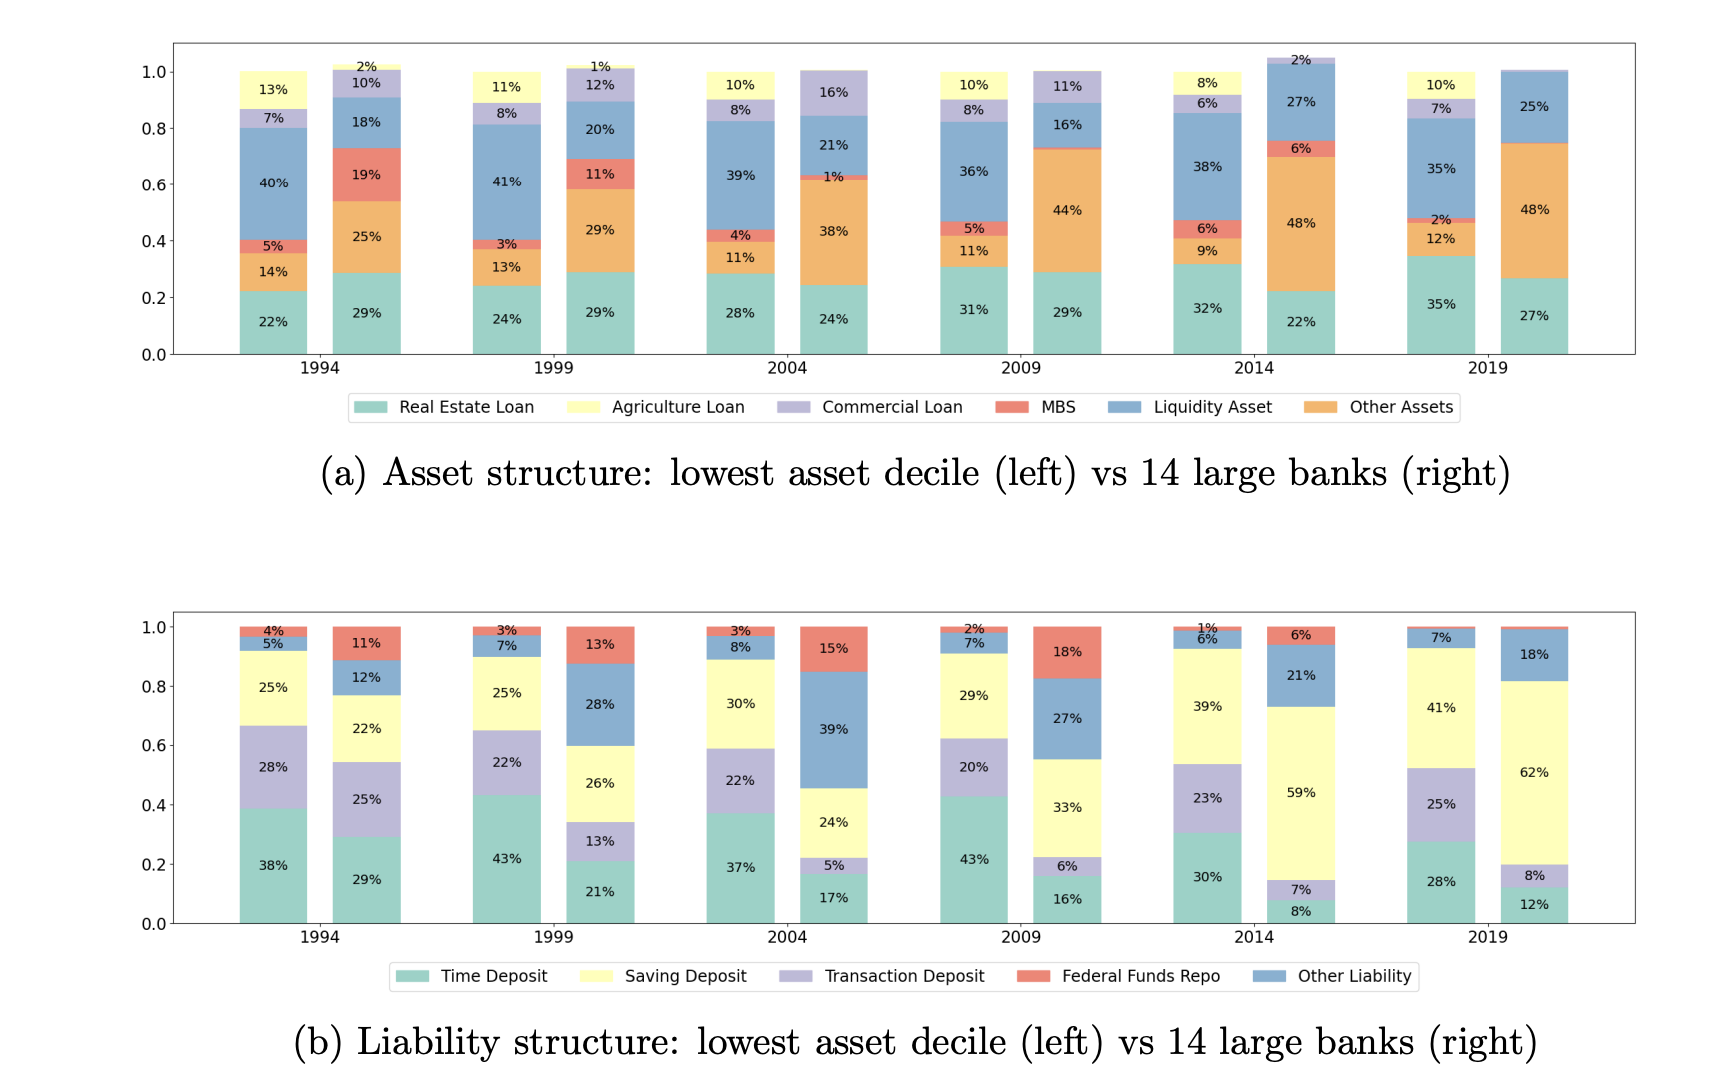
\includegraphics[width=0.99\textwidth]{imgs/fig7.png}
        %\caption*{Caption}
        \label{fig:my_label}
    \end{figure}
    
    \end{frame}



\begin{frame}{Evidence of spatial sorting}

    \begin{wideitemize}
        \item Define the average local population density of bank $j$ in state $s$ in year $t$ to be
        $$
        \log \left(\text { Density }_{j s t}\right)=\sum_{c \in \mathcal{C}_s}\left(\frac{b_{j c t}}{\sum_{c^{\prime} \in \mathcal{C}_s} b_{j c^{\prime} t}}\right) \log \left(\text { Density }_{c t}\right),
        $$

        where Density ${ }_{c t}$ is the population density of county $c$ in year $t, \mathcal{C}_s$ is the set of counties in state $s$, and $b_{j c t}$ is the number of branches of bank $j$ in county $c$ in year $t$. %We focus on sorting patterns within a given state in a given year. 
        
        \item  Main regression specification is
$$
\log \left(\text { Density }_{j s t}\right)=\beta \text { Size }_{j t}+\gamma_{s t}+\varepsilon_{j s t}
$$
where $\operatorname{Size}_{j t}$ is measured as log deposits of bank $j$ at time $t$ across all of its bank branches. 

\item[$\rightarrow$] $\beta>0$ coefficient is evidence of \textcolor{blue}{span-of-control sorting}.

\item[$\rightarrow$] Larger banks are located disproportionately in dense counties.

    \end{wideitemize}
%${ }^{38}$ We interpret a positive $\beta$ coefficient as evidence of span-of-control sorting, i.e. larger banks are located disproportionately in dense counties. Note that standard heterogeneous firm models, as in Melitz (2003), imply exactly the opposite. In those models, it is the productive firms that sell in the more marginal markets, which would imply a negative $\beta$ coefficient.
    \end{frame}

    \begin{frame}{Evidence of spatial sorting}

        \begin{figure}
            \centering
            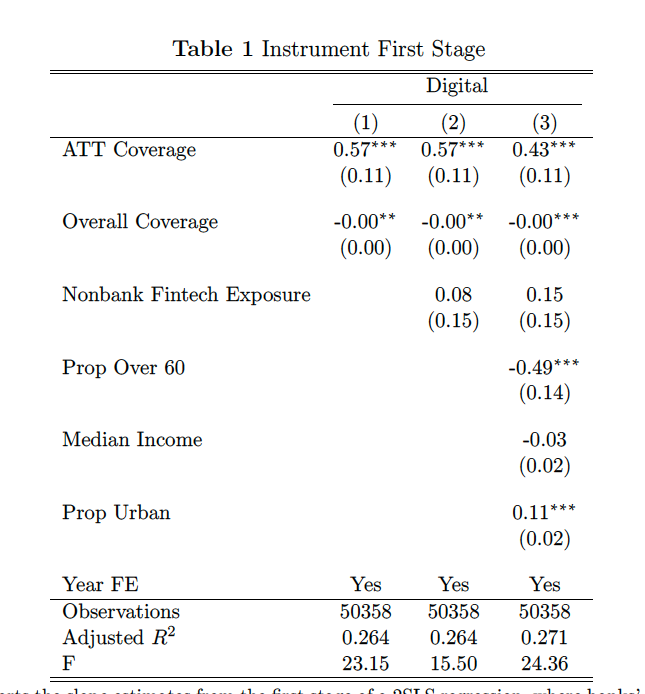
\includegraphics[width=0.8\textwidth]{imgs/tab1.png}
            \caption*{ Standard errors  
            are two-way clustered at the state and bank level.}
            \label{fig:my_label}
        \end{figure}
        
        \end{frame}
    


\begin{frame}{Evidence of spatial sorting: Role of distance}
    % the sample to banks that are active in two or more counties to avoid headquarters location biases. 
    
    \begin{wideitemize}
        \item   $\operatorname{dist}_{j s}^q=\mathbf{1}\left\{\log \left(\operatorname{dist}_{j s}\right)\right.$ in quartile $\left.q\right\}$ for $q=2,3,4$ and dist $_{j s}$ to be the avg dist. to HQ.  %We estimate the regression
        % \item %Define dist $_{j s}$ to be the average distance from bank $j$ 's headquarter county to its branches in state $s$, and
    $$
    \log (\text { Density })_{j s t}=\beta \operatorname{Size}_{j t}+\sum_{q=2}^4 \theta_q \operatorname{dist}_{j s}^q+\sum_{q=2}^4 \beta_q \operatorname{Size}_{j t} \times \operatorname{dist}_{j s}^q+\gamma_{s t}+\varepsilon_{j s t} .
    $$
    \item Sorting declines with distance and faraway banks are in more dense counties. 

    \end{wideitemize}
    \begin{figure}
        \centering
        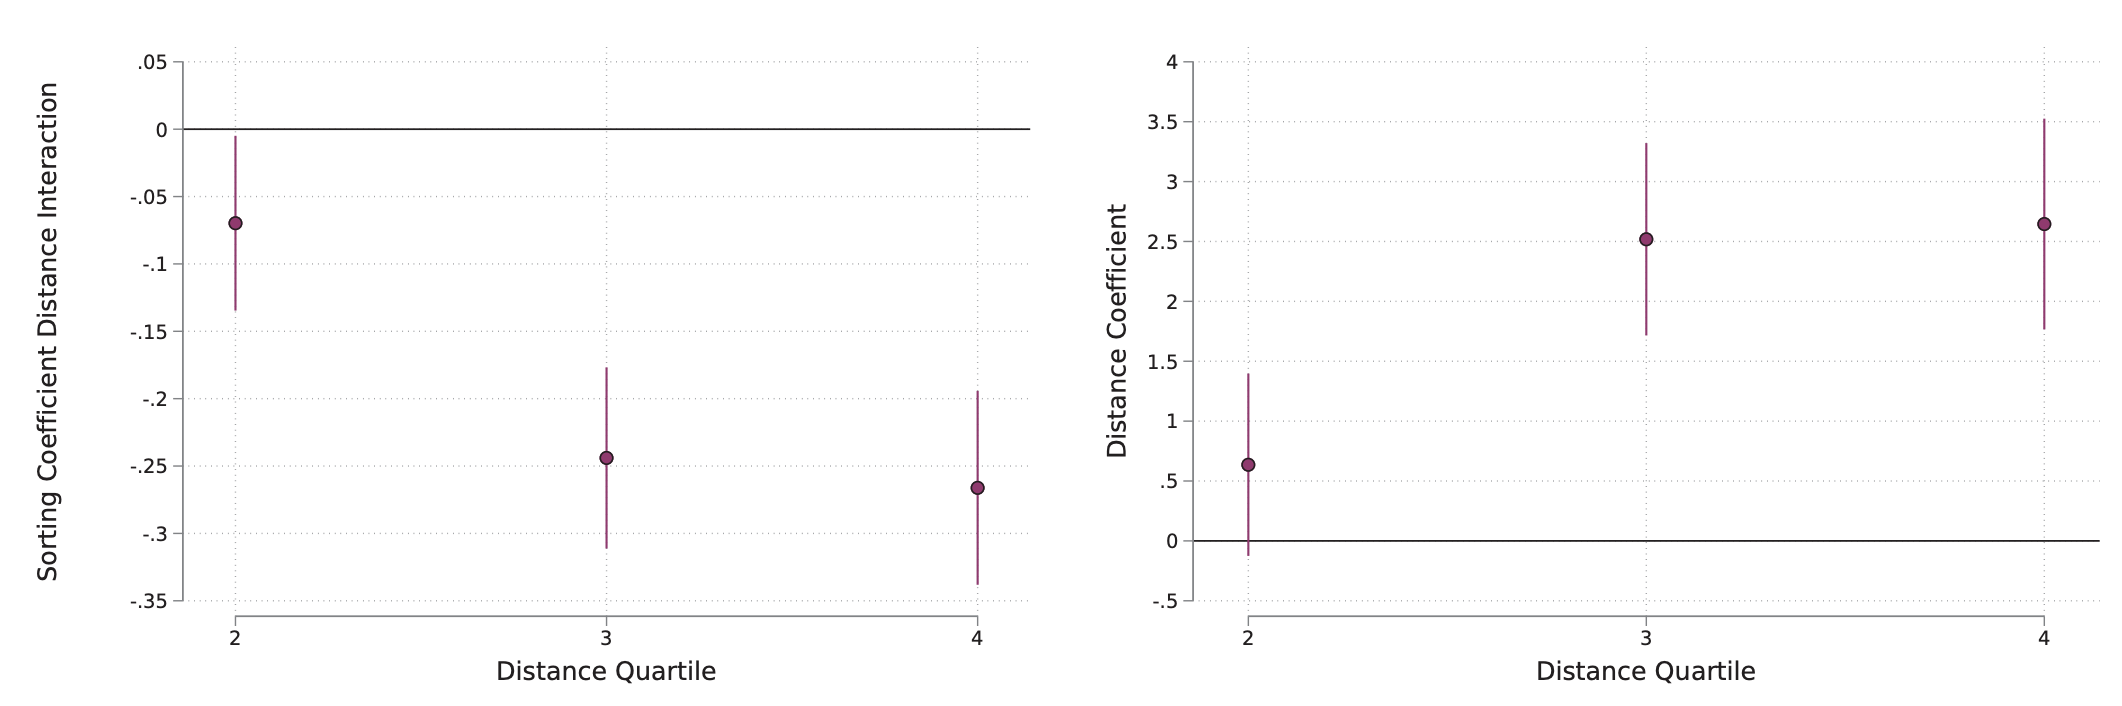
\includegraphics[width=0.8\textwidth]{imgs/fig8.png}
        \caption*{Changes in relative and absolute sorting patterns between 1981 and 2006 for
        four bank-size bins.\\ (a) Sorting interaction coefficients. (b) Distance coefficients.}
        % (b) Distance coefficients.}
        \label{fig:my_label}
    \end{figure}

    % \begin{itemize}
  
    % \end{itemize}


    
    \end{frame}


    \begin{frame}{Evidence of spatial sorting}
    
    % granular geographic approach to understand the determinants of branching in particular
    % counties. For example, do large banks expand into cities relatively more than small banks? Does the distance
    % between a bank and its target county have a measured effect on the number of branches they choose to set
\begin{wideitemize}
    \item Estimate the Poisson regression
$$
\log \left(\mathbb{E}\left[\operatorname{Branches}_{j c t}\right]\right)=\underbrace{\delta \operatorname{Size}_{j t} \times \log \left(\operatorname{Density}_{c t}\right)}_{\text {sorting motives }}+\underbrace{\theta \log \left(\operatorname{Miles}_{j c}\right)}_{\text {distance effect }}+\gamma_{c t}+\gamma_{j t}+\varepsilon_{j c t} .
$$

\begin{wideitemize}
    \item where Branches $_{j c t}$ is the total number of branches of bank $j$ in county $c$ in year $t$,
    \item Miles${ }_{j c}$ is the distance in miles from centroid of bank $j$ 's headquarter county and the centroid of $c$. 
    \item Standardize both bank size and log county population density.
    
    %We interpret a positive $\delta$ estimate as evidence for spatial span-of-control sorting: large banks have more branches, but especially so in dense counties.
% where Branches $_{j c t}$ denotes the total number of branches of bank $j$ in county $c$ in year $t$ and Miles ${ }_{j c}$ is the distance in miles from the centroid of bank $j$ 's headquarter county and the centroid of county $c$. 
% We standardize both bank size and log county population density. We interpret a positive $\delta$ estimate as evidence for spatial span-of-control sorting: large banks have more branches, but especially so in dense counties.

% We limit our sample to banks that at some point in the sample were active in 35 or more counties. We do this for two reasons. First, with over 3,000 counties and 26 years, each bank year in the data consists of nearly 80,000 observations. With about 9,000 banks per year on average, this gives over 250 million

\end{wideitemize}

\item[$\rightarrow$] $\delta>0$ coefficient is evidence of \textcolor{blue}{span-of-control sorting}.
\item[$\rightarrow$] Larger banks have more branches, but especially so in dense counties.

\end{wideitemize}
    \end{frame}

    \begin{frame}{Evidence of spatial sorting}
    
        \begin{figure}
            \centering
            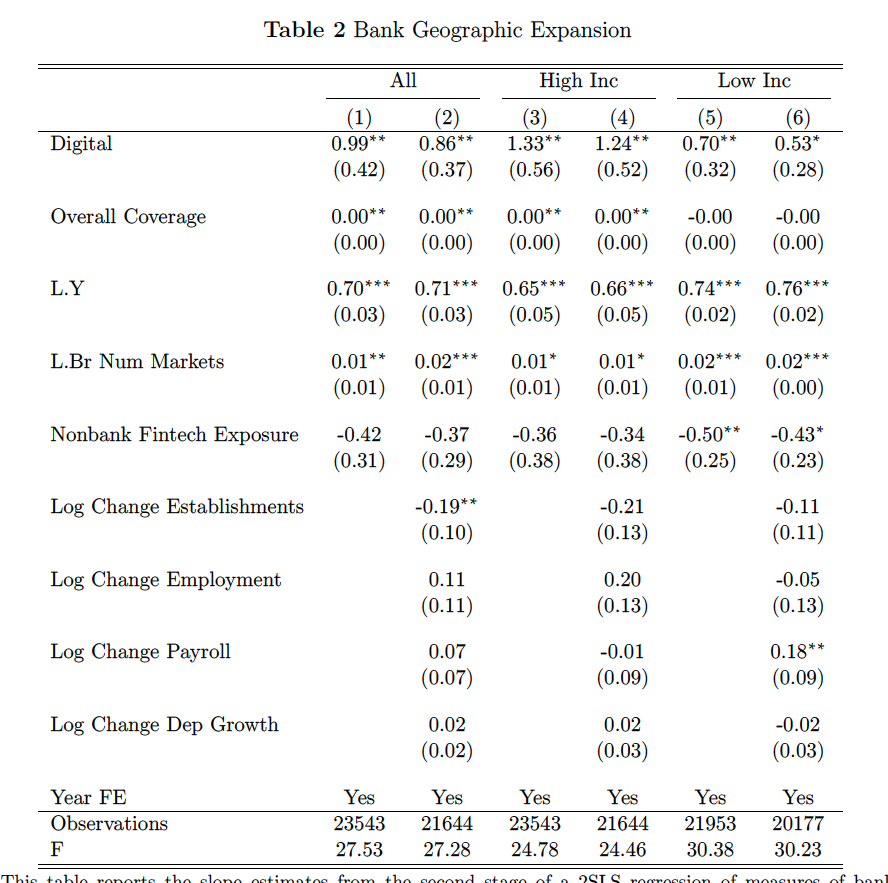
\includegraphics[width=0.78\textwidth]{imgs/tab2.png}
            \caption*{Heteroscedasticity-robust standard
            errors are reported in parentheses}
            \label{fig:my_label}
        \end{figure}
        
        \end{frame}


        \begin{frame}{Sorting over time and impact of deregulation}
            \begin{wideitemize}
                %How did this expansion affect spatial sorting patterns? 
                \item Top 1\% of banks grew in the densest counties, but lost branch share in the most dense counties. 
                % \item Top 1\% of banks grew in the least dense counties, but lost branch share in the least dense counties.
        \end{wideitemize}

    \begin{figure}
        \centering
        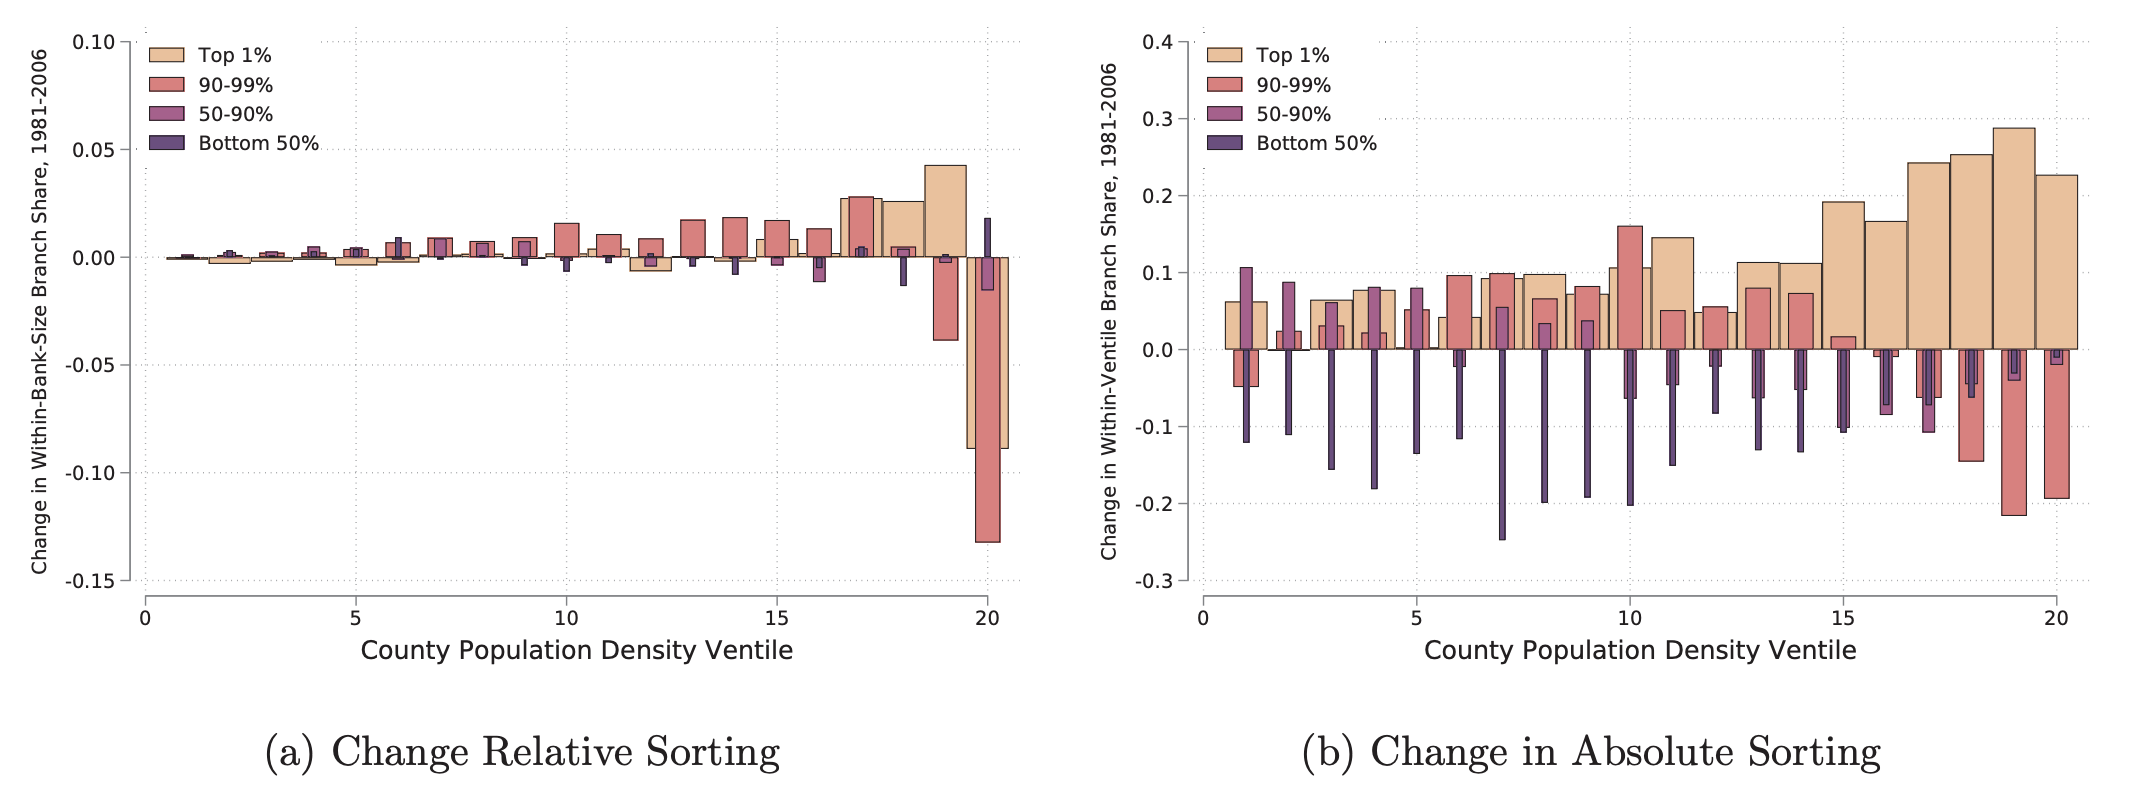
\includegraphics[width=0.99\textwidth]{imgs/fig9.png}
        \caption*{
            Pattern cheange between 1981 and 2006 by county density and bank size. }
        \label{fig:my_label}
        % notes here
    \end{figure}

    % Patterns between 1981 and 2006 by county density and bank size. 
    
    \end{frame}

    \begin{frame}{Sorting over time and impact of deregulation}\label{sorting_time}
    % to study this empirical finding in more detail. In particular, we explore how sorting changed over time using our regression analysis. We begin by estimating equation (17) year by year to allow the sorting coefficient to vary over time. Namely, we estimate
    \begin{itemize}
        \item Decline in relative sorting patterns until 1998.  %, after which the sorting estimates plateau.
% button to stag time 
\hyperlink{stag_time}{\beamerbutton{Staggered changes}}
    
    $$
    \log (\text { Density })_{j s t}=\beta_t \text { Size }_{j t}+\gamma_{s t}+\varepsilon_{j s t}, \quad t=1981, \ldots, 2006 .
    $$
    \end{itemize}
    
    % Figure 10a shows the evolution of the density-size sorting elasticity over time. There is a consistent decline in relative sorting patterns until 1998, after which the sorting estimates plateau. The decline is significant: the coefficient falls from 0.37 in 1981 to an average of 0.22 after 1998.
    
    % Figure 10b connects the decline in sorting to geographic deregulation. We plot the estimated sorting coefficient from equation (20) against the average number of reciprocal agreements per state in a given year. There is a clear negative trend: in the early stages of deregulation, sorting estimates are clustered around 0.33 . As the deregulation picked up, there is a clear decline, culminating at the 0.22 level following the passage of the IBBEA, when all states deregulated fully.
    \begin{figure}
        \centering
        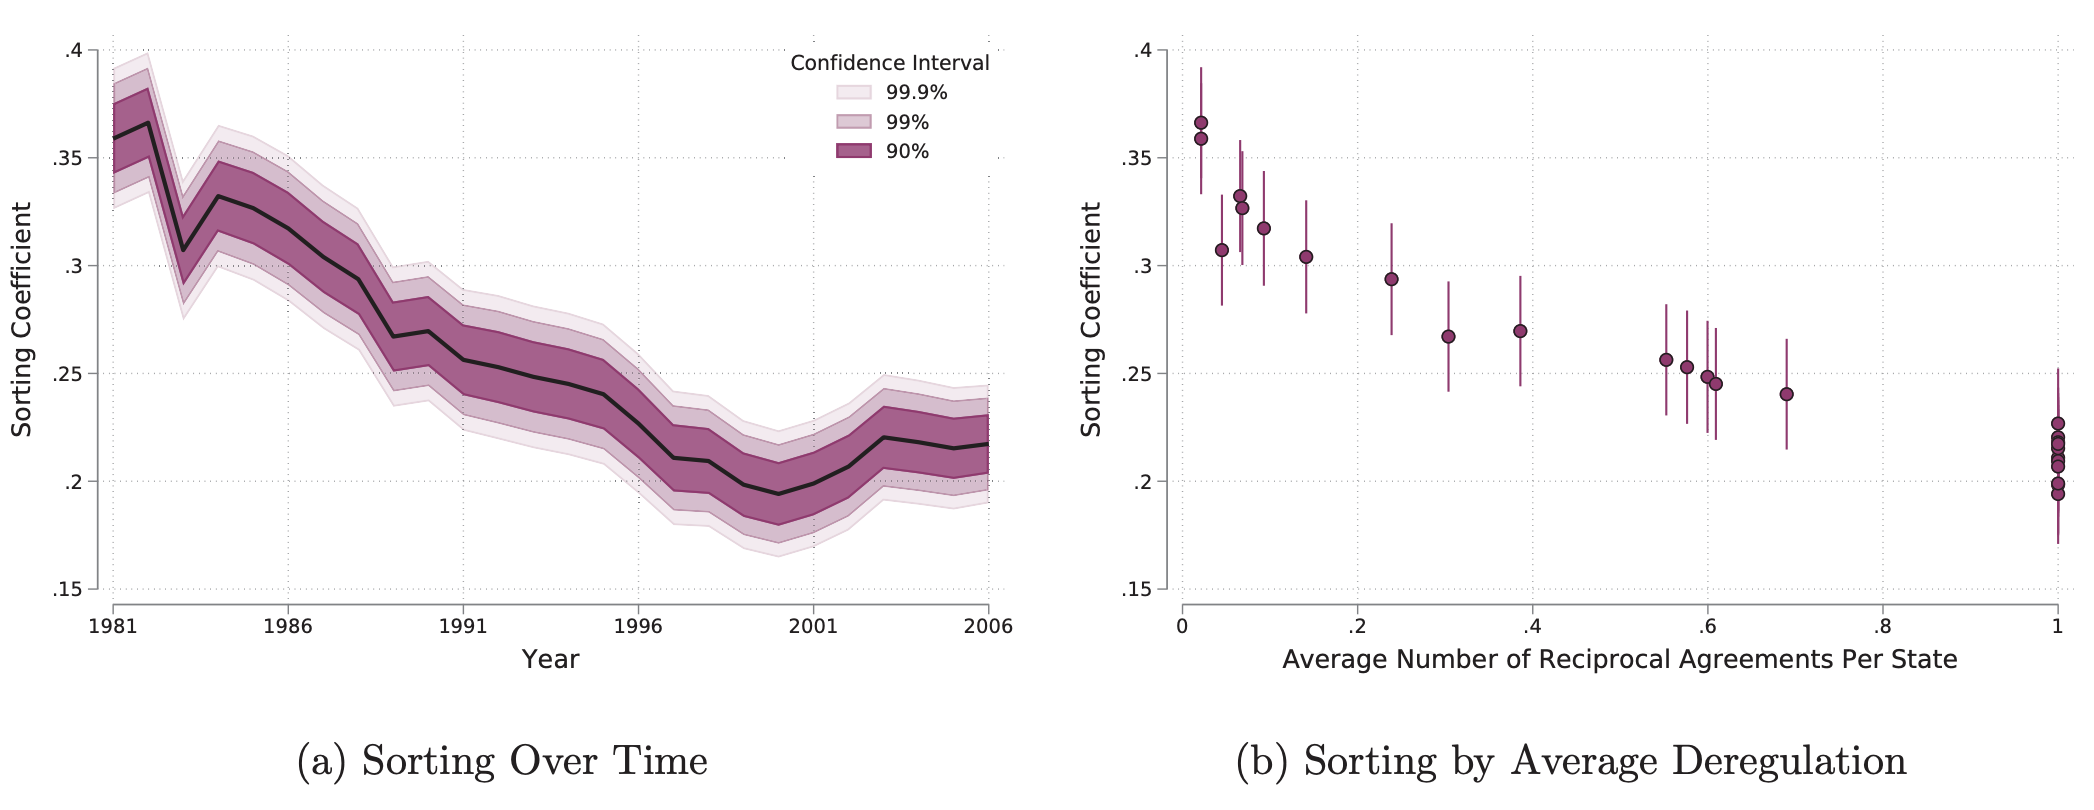
\includegraphics[width=0.99\textwidth]{imgs/fig10.png}
        \caption*{Sorting coefficients $\beta_t$ between 1981 and 2006.}
        \label{fig:my_label}
    \end{figure}
    
    \end{frame}

    

        \begin{frame}{Sorting over time and impact of deregulation: Event study}
            \begin{itemize}
                \item Weakened sorting patterns after deregulation. %, after which the sorting estimates plateau.
    
            
            %Of course, we cannot rule out that the estimation may be simply picking up pre-trends in sorting patterns. Many states deregulated in-state branching in the late 1970s and early 1980s, which could drive changes in sorting patterns as banks became less geographically constrained within a given state. %We therefore further test for causality by looking at the dynamic effects of deregulation on sorting. We estimate an event study specification given by
            $$
            \log \left(\text { Density }_{j s t}\right)=\beta \operatorname{Size}_{j t}+\sum_{\substack{-5 \leq h \leq 10 \\ h \neq-1}} \beta_h \operatorname{Size}_{j t} \times \text { Open }_{s t+h}+\gamma_{s t}+\varepsilon_{j s t},
            $$
            where $\operatorname{Open}_{s t+h}$ is equal to 1 if $\operatorname{Recip}_{s t+h}>0$, $h=0$ the first period in which a state opened up.
        \end{itemize}
    %Of course, we cannot rule out that the estimation may be simply picking up pre-trends in sorting patterns. Many states deregulated in-state branching in the late 1970s and early 1980s, which could drive changes in sorting patterns as banks became less geographically constrained within a given state. %We therefore further test for causality by looking at the dynamic effects of deregulation on sorting. We estimate an event study specification given by
    % $$
    % \log \left(\text { Density }_{j s t}\right)=\beta \operatorname{Size}_{j t}+\sum_{\substack{-5 \leq h \leq 10 \\ h \neq-1}} \beta_h \operatorname{Size}_{j t} \times \text { Open }_{s t+h}+\gamma_{s t}+\varepsilon_{j s t},
    % $$
    % where $\operatorname{Open}_{s t+h}$ is an indicator equal to 1 if $\operatorname{Recip}_{s t+h}>0$. We let $h=0$ refer to the first period in which a state opened up to any other state. 
    %If the results in Table III are driven by changes in sorting induced by intra-state branching deregulation, then the pre-trend coefficients $(h<0)$ should be positive.
    
    % Figure 11 plots the results of the event study. The pre-trend coefficients average 0.01 and are all statistically insignificant at the $5 \%$ level. All of the post-opening coefficients are negative, and only the initial deregulation year is insignificant. The effects are monotonically declining over time following the initial opening, which likely reflects the increasing degree of openness over time.
    \begin{figure}
        \centering
        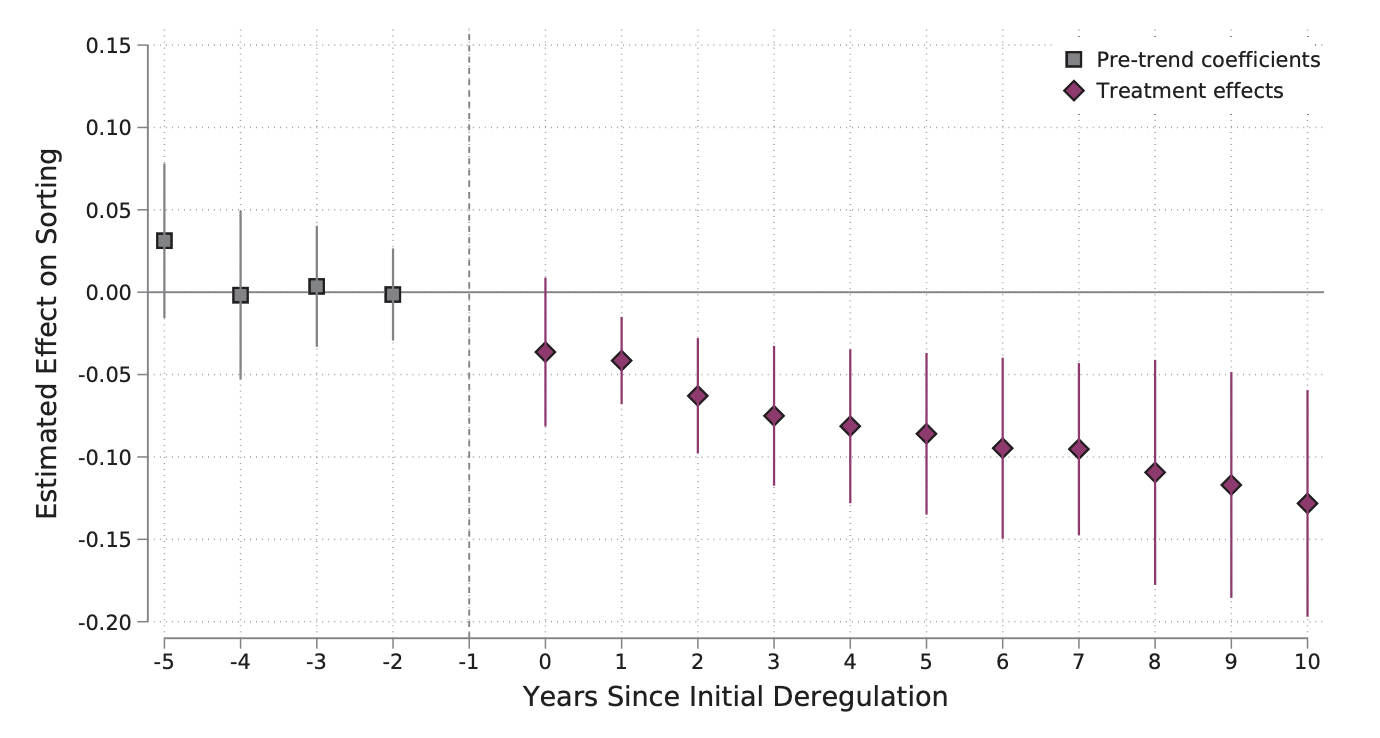
\includegraphics[width=0.6\textwidth]{imgs/fig11.png}
        %\caption*{Caption}
        \label{fig:my_label}
        \caption*{Standard errors are two-way clustered at the state and bank level.}
    \end{figure}
    
    \end{frame}



    \begin{frame}{Connecting mismatch sorting to the level of wholesale funding}\label{mismatch_sorting}

        \vspace{0.1cm}

        \textcolor{blue}{Mismatch sorting:} Banks choose locations based on the match of the location's characteristics to the funding needs.
        %! Summary of the results
        \begin{wideitemize}
            \item Denser locations are less deposit intensive \hyperlink{mismatch_sorting1}{\beamerbutton{Regression}}
            
            \item Banks that were headquartered in counties with more loan opportunities used more wholesale funding in 1984. 
            \hyperlink{mismatch_sorting2}{\beamerbutton{Regression}}
            
            \item Banks with more exposure to wholesale funding expanded into locations that were deposit-abundant.
            \hyperlink{mismatch_sorting3}{\beamerbutton{Poisson regression}}

        \end{wideitemize}
            
        
        \end{frame}

        \begin{frame}{The impact of deregulation on bank expansion and wholesale funding}\label{der_impact}
            \begin{wideitemize}
                \item What was the effect of expansion on the dynamics of a bank’s reliance on wholesale funding? % after the deregulation?S
                
                \item Regress the change in a bank's outcome variable on WSF. \hyperlink{der_impact1}{\beamerbutton{Specification details}}
            \item Results:
            \vspace{0.2cm}
                \begin{wideitemize}
        \item Large firms decrease their wholesale funding
        exposure immediately after deregulation. %The effect grows over time and stabilizes.

        \item  Number of branches and active counties have positive cumulative effects from wholesale funding. 

        \item Geographic deregulation relaxed liquidity constraints for banks,
        allowing them to raise deposits through branching and reduce their exposure to wholesale
        funding. 

            \end{wideitemize}
                
            \end{wideitemize}

              
    \end{frame}
    

\begin{frame}{The impact of deregulation on bank expansion and wholesale funding}\label{der_impac2}
    \begin{itemize}
        \item What was the effect of expansion on the dynamics of a bank’s reliance on wholesale funding? % after the deregulation?
         \end{itemize}
        % We have already shown that banks that started with wholesale funding expanded into less dense locations that were more deposit-abundant. The final step is to explore what was the effect of this expansion on the dynamics of a bank's overall reliance on wholesale funding after the deregulation shock. We do this by studying the dynamics of the deregulation shock on a bank's geographic expansion and wholesale funding reliance as a function of the bank's initial size and wholesale funding use. Let Large ${ }_j$ be an indicator equal to 1 if bank $j$ is in the top $5 \%$ of banks by deposits in the first sample year, 1984. Given an outcome variable $Y_{j t}$, we estimate

        % for $h=1, \ldots, 7 $ 
        %We consider the relative effect of differential use of wholesale funding, $\mathrm{WFE}_{j t}$ and $\mathrm{WFE}_{j^{\prime} t}$, for two banks with identical expansion options, $\operatorname{Recip}_{j t}=$ Recip $_{j^{\prime} t}$, in an identical size bin, Large $_j=$ Large $_{j^{\prime}}$. The differential effect on outcome $Y_{(\cdot)}$ at horizon $h$ of total deregulation, Recip ${ }_{j t}=1$, is then given by $\left[\beta_{1 h}+\beta_{3 h}\right.$ Large $\left._j\right]\left(\mathrm{WFE}_{j t}-\mathrm{WFE}_{j^{\prime} t}\right)$. We consider three dependent variables: wholesale funding exposure, total branches, and total counties with at least one branch. We plot the effects for each measure given a one standard deviation increase in wholesale funding for small (below top $5 \%$ in deposits) and large (above top $5 \%$ in deposits) banks. The standard deviations of wholesale funding are 0.099 and 0.149 , respectively.


    \begin{figure}
        \centering
        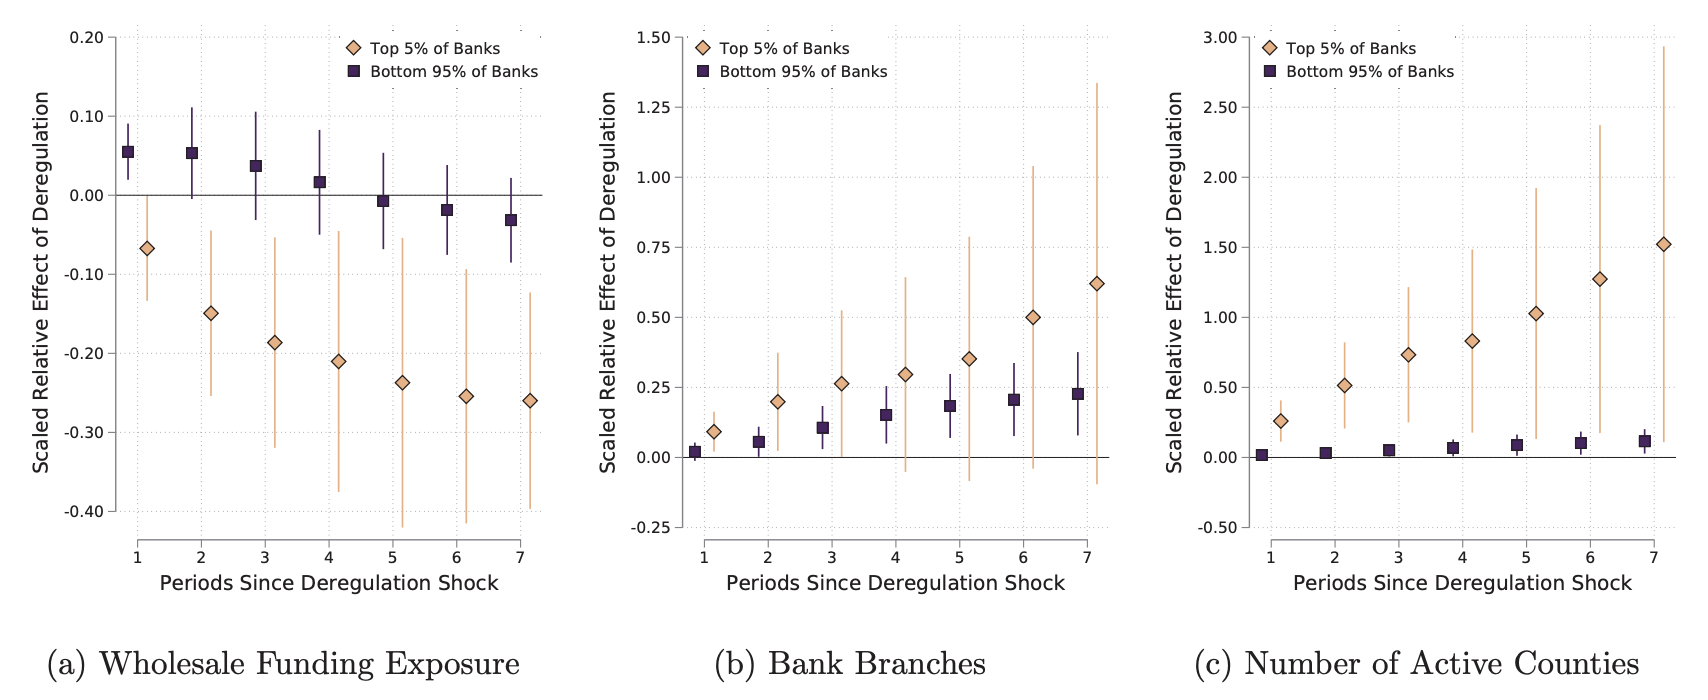
\includegraphics[width=0.99\textwidth]{imgs/fig12.png}
        %\caption*{Caption}
        \label{fig:my_label}
    \end{figure}
    
    \end{frame}

% Conclusion frame
\begin{frame}{Conclusion}
    % \begin{wideitemize}
        % \item \textcolor{blue}{Summary:} 
        \begin{wideitemize}

            \item Paper proposes a model of spatial sorting of banks.
    
            \item Banks sort into locations based on mismatch sorting and span-of-control sorting.
            % \item Span-of-control sorting: more productive banks sort into denser locations.
            \item Evidence evidence seems to support the model.
            \item Deregulation relaxed liquidity constraints for banks through branching.
        \end{wideitemize}
        % \item \textcolor{blue}{Contribution:} 
        % \begin{wideitemize}
        %     \item Study the impact of deregulation on bank expansion and wholesale funding.
        %     \item Connect mismatch sorting to the level of wholesale funding.
        % \end{wideitemize}
        % \item \textcolor{blue}{Policy implications:} 
        % \begin{wideitemize}
        %     \item Deregulation relaxed liquidity constraints for banks.
        %     \item Banks with more exposure to wholesale funding expanded into locations that were deposit-abundant.
        % \end{wideitemize}
    % \end{wideitemize}
    \end{frame}
    

    \begin{frame}{}
        % Thank you slide
        \centering
        \huge \textcolor{blue}{Thank you!}
    \end{frame}


    \appendix

    % appendix slides
    \begin{frame}[noframenumbering]
        \centering
        \huge \textcolor{blue}{Appendix}
    \end{frame}

    \begin{frame}{Impact of deregulation: Staggered changes in deregulation\hyperlink{sorting_time}{\beamerbutton{back}}
        }\label{stag_time}

    \begin{figure}
        \centering
            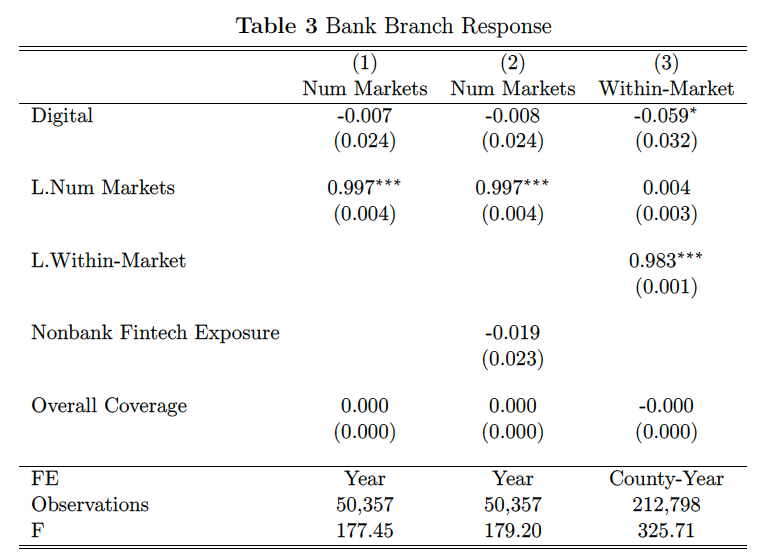
\includegraphics[width=0.8\textwidth]{imgs/tab3.png}
            %\caption*{Caption}
            \label{fig:my_label}
        \end{figure}
        
        \end{frame}
    

        \begin{frame}{Connecting mismatch sorting to the level of wholesale funding         \hyperlink{mismatch_sorting}{\beamerbutton{Back}}}\label{mismatch_sorting1}

            % back button to mismatch sorting 
    
            \vspace{0.1cm}
            \begin{itemize}
                \item Denser locations are less deposit intensive.
            % county density. To investigate this pattern we estimate a county-level regression given by
    $$
    \log (D / L)_{c t}=\phi \log \left(\text { Density }_{c t}\right)+\operatorname{controls~}_{c t}+\gamma_t+\varepsilon_{c t}
    $$
    % where $\log (D / L)_{c t}$ denotes the log of the deposits to loans ratio in county $c$ at time $t$. 
    \end{itemize}
    %If $\phi<0$, then low-density counties have on average more deposits than loans relative to high-density counties, corroborating the pattern required for mismatch sorting to reduce overall sorting in response to geographic deregulation. We progressively include controls in the regression, such as county per-capita income and the number of local banks and branches. We also consider a specification with state-year fixed effects to control for differences in financial development across states and to better connect the results to the sorting regressions in the previous section. Table IV reports the results. In all specifications, we find $\phi<0$, implying that low-density counties are more deposit-intensive relative to high-density counties. ${ }^{44}$
            \begin{figure}
                \centering
                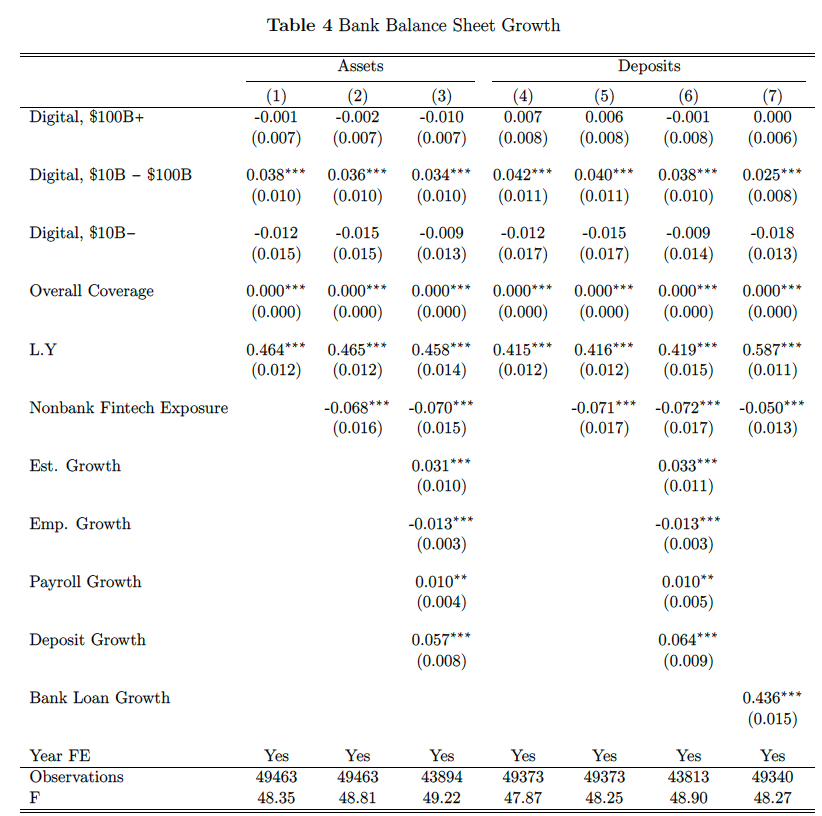
\includegraphics[width=0.71\textwidth]{imgs/tab4.png}
                \caption*{Heteroscedasticity-robust standard errors are reported in parentheses.}
                \label{fig:my_label}
            \end{figure}
            
            \end{frame}
    
    
            \begin{frame}{Headquarter location and the use of wholesale funding         \hyperlink{mismatch_sorting}{\beamerbutton{Back}}}\label{mismatch_sorting2}
    % \begin{frame}{Spatial expansion patterns and the level of wholesale funding}
        %Having established that, we now study if banks that were headquartered in counties with relatively more loan opportunities used more wholesale funding. To do so, we estimate
        \begin{itemize}
            \item Less wholesale funding in counties that are deposit intensive.
            $$
            \mathrm{WFE}_{j, 1984}=\beta \log (D / L)_{c_j^{H Q}}+\operatorname{controls}_{j, 1984}+\varepsilon_{j, 1984} .
            $$
            where $\mathrm{WFE}_{j, 1984}$ denotes the log of bank $j$ 's wholesale funding exposure in 1984. % and $\log (D / L)_{c_j^{H Q}}$ is our measure of deposits to loans for bank $j$ 's headquarter county. 
        \end{itemize}
    
        
        %${ }^{45}$ We gradually add controls for the density of a bank's headquarters county and the size of the bank. We present the results in Table V.
        \begin{figure}
            \centering
            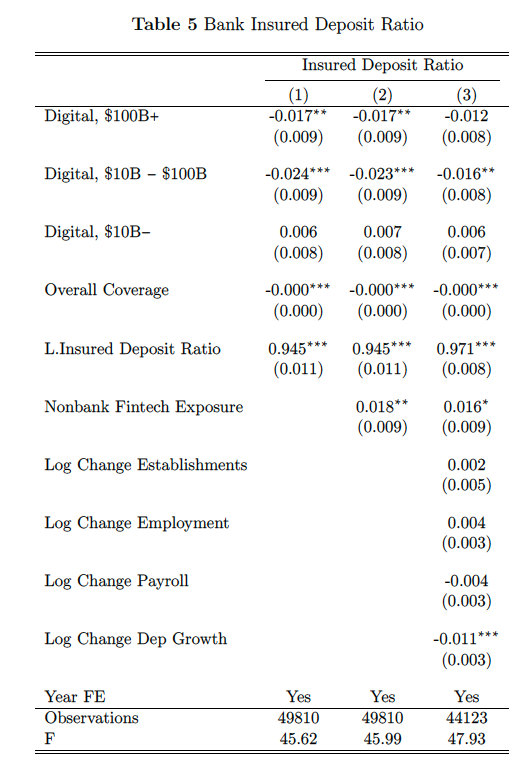
\includegraphics[width=0.75\textwidth]{imgs/tab5.png}
            %\caption*{Caption}
            \label{fig:my_label}
        \end{figure}
        
        \end{frame}
    
    
    
        \begin{frame}{Spatial expansion patterns and the level of wholesale funding         \hyperlink{mismatch_sorting}{\beamerbutton{Back}}}\label{mismatch_sorting3}
    
        \begin{wideitemize}
            \item
     Estimate the Poisson regression:
            $$
            \begin{aligned}
            \log \left(\mathbb{E}\left[\text { branches }_{j c t}\right]\right)= & \beta_0 \mathrm{WFE}_{j, 1984} \times \log (D / L)_c+\beta_1 \mathrm{WFE}_{j, 1984} \times \log \left(\text { Density }_{c t}\right) \\
            & +\phi_0 \operatorname{Size}_{j t} \times \log (D / L)_c+\phi_1 \operatorname{Size}_{j t} \times \log \left(\text { Density }_{c t}\right) \\
            & +\delta \log \left(\text { Dist }_{j c}\right)+\gamma_{j t}+\gamma_{c t}+\varepsilon_{j c t} .
            \end{aligned}
            $$
            
            % Our coefficient of interest is $\beta_0$, which measures the relative propensity of firms with higher levels of wholesale funding to expand into deposit-intensive locations. We include the remaining terms to control for the possibility that expansion decisions are driven by size and density alone. As in previous regressions, we
    
            \item[$\rightarrow$] Banks with more exposure to wholesale funding expanded into locations that were deposit-abundant. % over this period. To test this,
        \end{wideitemize}
            
    
        % \begin{figure}
        %     \centering
        %     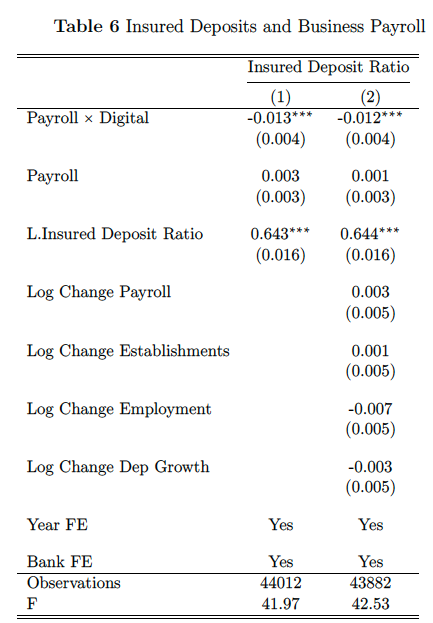
\includegraphics[width=0.6\textwidth]{imgs/tab6.png}
        %     %\caption*{Caption}
        %     \label{fig:my_label}
        % \end{figure}
        
        \end{frame}
    
    
    
    
        \begin{frame}{Spatial expansion patterns and the level of wholesale funding         \hyperlink{mismatch_sorting}{\beamerbutton{Back}}}\label{mismatch_sorting4}
    
        %     \begin{wideitemize}
        %         \item
        %  Estimate the Poisson regression:
        %         $$
        %         \begin{aligned}
        %         \log \left(\mathbb{E}\left[\text { branches }_{j c t}\right]\right)= & \beta_0 \mathrm{WFE}_{j, 1984} \times \log (D / L)_c+\beta_1 \mathrm{WFE}_{j, 1984} \times \log \left(\text { Density }_{c t}\right) \\
        %         & +\phi_0 \operatorname{Size}_{j t} \times \log (D / L)_c+\phi_1 \operatorname{Size}_{j t} \times \log \left(\text { Density }_{c t}\right) \\
        %         & +\delta \log \left(\text { Dist }_{j c}\right)+\gamma_{j t}+\gamma_{c t}+\varepsilon_{j c t} .
        %         \end{aligned}
        %         $$
                
        %         % Our coefficient of interest is $\beta_0$, which measures the relative propensity of firms with higher levels of wholesale funding to expand into deposit-intensive locations. We include the remaining terms to control for the possibility that expansion decisions are driven by size and density alone. As in previous regressions, we
        
        %         \item[$\rightarrow$] Banks with more exposure to wholesale funding expanded into locations that were deposit-abundant. % over this period. To test this,
        %     \end{wideitemize}
                
        
            \begin{figure}
                \centering
                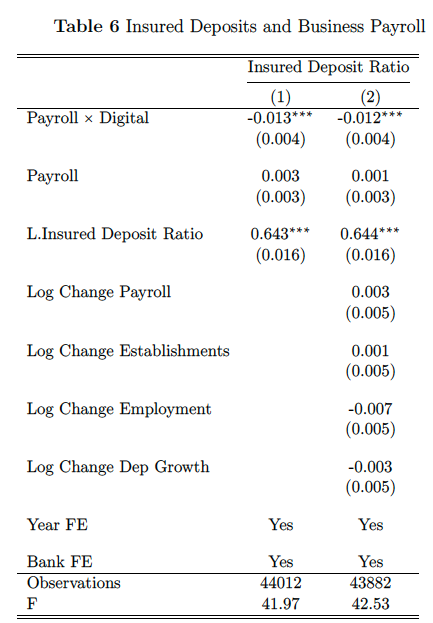
\includegraphics[width=0.6\textwidth]{imgs/tab6.png}
                %\caption*{Caption}
                \label{fig:my_label}
            \end{figure}
            
            \end{frame}
        
    
        \begin{frame}{Spatial expansion patterns and the level of wholesale funding}\label{mismatch_sorting5}
    
            %To complement this evidence, we explore how wholesale funding exposure prior to deregulation affected the expansion and sorting decisions on banks along the deposits-to-loans $(D / L)$ margin. To do so, we estimate the regression
            $$
            \log (D / L)_{j s t}=\beta_0 \operatorname{Size}_{j t}+\beta_1 \operatorname{Size}_{j t} \times \operatorname{Recip}_{s t}+\beta_2 \mathrm{WFE}_{j, 1984}+\beta_3 \mathrm{WFE}_{j, 1984} \times \operatorname{Recip}_{s t}+\gamma_{s t}+\varepsilon_{j s t}
            $$
            % where $\log (D / L)_{j s t}$ denotes the branch-weighted average of county-level deposit-to-loan ratios for each bank in each year.%
        \begin{figure}
            \centering
            \caption*{{Standard errors are reported in parentheses and are two-way clustered at the state and
            bank level.}}
            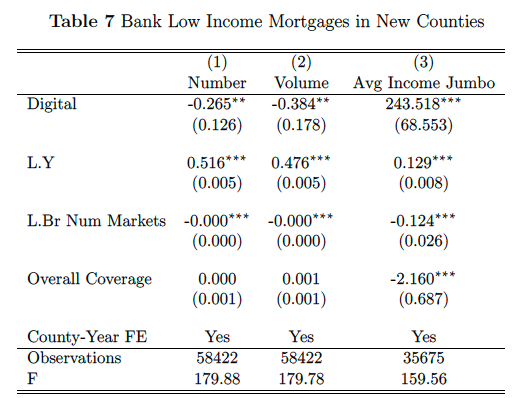
\includegraphics[width=0.74\textwidth]{imgs/tab7.png}
            \label{fig:my_label}
        \end{figure}
        
        \end{frame}
    

        \begin{frame}{The impact of deregulation on bank expansion and wholesale funding \hyperlink{der_impact}{\beamerbutton{Back}}
            }\label{der_impact1}
            \begin{itemize}
                \item What was the effect of expansion on the dynamics of a bank’s reliance on wholesale funding? % after the deregulation?
     
                % We have already shown that banks that started with wholesale funding expanded into less dense locations that were more deposit-abundant. The final step is to explore what was the effect of this expansion on the dynamics of a bank's overall reliance on wholesale funding after the deregulation shock. We do this by studying the dynamics of the deregulation shock on a bank's geographic expansion and wholesale funding reliance as a function of the bank's initial size and wholesale funding use. Let Large ${ }_j$ be an indicator equal to 1 if bank $j$ is in the top $5 \%$ of banks by deposits in the first sample year, 1984. Given an outcome variable $Y_{j t}$, we estimate
                \item Regress the change in a bank's outcome variable on the change in wholesale funding.
    
                %We consider the relative effect of differential use of wholesale funding, $\mathrm{WFE}_{j t}$ and $\mathrm{WFE}_{j^{\prime} t}$, for two banks with identical expansion options, $\operatorname{Recip}_{j t}=$ Recip $_{j^{\prime} t}$, in an identical size bin, Large $_j=$ Large $_{j^{\prime}}$. The differential effect on outcome $Y_{(\cdot)}$ at horizon $h$ of total deregulation, Recip ${ }_{j t}=1$, is then given by $\left[\beta_{1 h}+\beta_{3 h}\right.$ Large $\left._j\right]\left(\mathrm{WFE}_{j t}-\mathrm{WFE}_{j^{\prime} t}\right)$. We consider three dependent variables: wholesale funding exposure, total branches, and total counties with at least one branch. We plot the effects for each measure given a one standard deviation increase in wholesale funding for small (below top $5 \%$ in deposits) and large (above top $5 \%$ in deposits) banks. The standard deviations of wholesale funding are 0.099 and 0.149 , respectively.
        
            \end{itemize}
    
            $$
            \begin{aligned}
            Y_{j t+h}-Y_{j t}=\underbrace{\beta_{0 h} \operatorname{Recip}_{j t}}_{\begin{array}{c}
            \text { baseline } \\
            \text { effect }
            \end{array}}+\underbrace{\beta_{1 h} \operatorname{Recip}_{j t} \times \mathrm{WFE}_{j t}}_{\begin{array}{c}
            \text { additional effect } \\
            \text { of wholesale funding }
            \end{array}} & +\underbrace{\beta_{2 h} \operatorname{Recip}_{j t} \times \operatorname{Large}_j}_{\begin{array}{c}
            \text { additional } \\
            \text { size effect }
            \end{array}}\\
             & +\underbrace{\beta_{3 h} \operatorname{Recip}_{j t} \times \mathrm{WFE}_{j t} \times \operatorname{Large}_j}_{\begin{array}{c}
            \text { additional size effect } \\
            \text { of wholesale funding }
            \end{array}} \\
            & +\beta_{4 h} \mathrm{WFE}_{j t}+\beta_{5 h} \mathrm{WFE}_{j t} \times \operatorname{Large}_j+\gamma_t+\gamma_j+\varepsilon_{j t}
            \end{aligned}
            $$
    
    
            where  $h=1, \ldots, 7 $, $\operatorname{Large}_j$ is equal to 1 if bank $j$ is in the top $5 \%$ of banks by deposits in the first sample year, 1984; $\operatorname{Recip}_{j t}$ is equal to 1 if bank $j$ is in a state that has opened up to any other state by year $t$. %and $\mathrm{WFE}_{j t}$ is the log of bank $j$ 's wholesale funding exposure in year $t$.
            % \begin{figure}
            %     \centering
            %     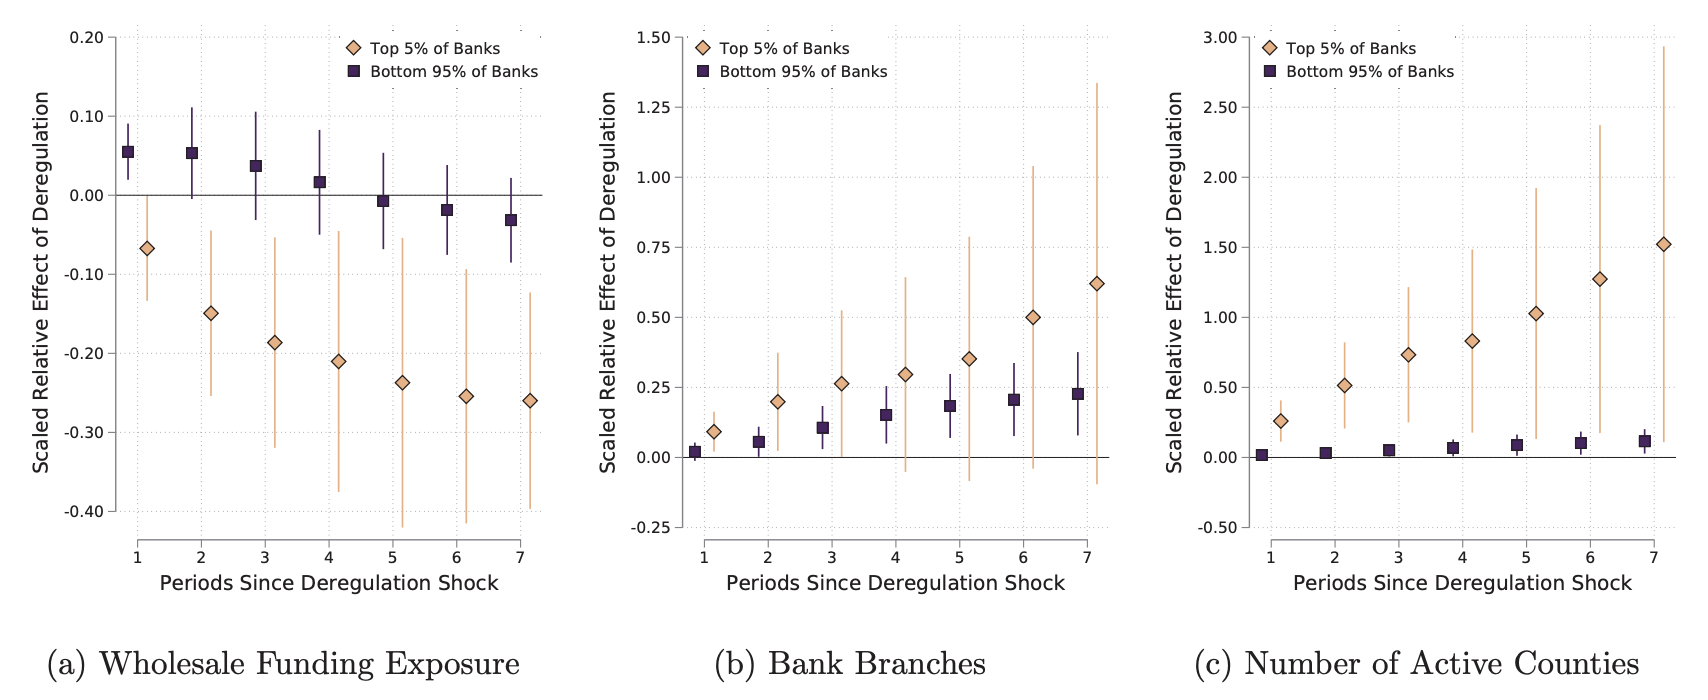
\includegraphics[width=0.99\textwidth]{imgs/fig12.png}
            %     %\caption*{Caption}
            %     \label{fig:my_label}
            % \end{figure}
            
            \end{frame}
        

\end{document}